\documentclass{article}
\usepackage[document]{ragged2e}
\usepackage[portuguese]{babel}
\usepackage{booktabs}
\usepackage[a4paper, left=3cm, right=1.5cm, top=3cm, bottom=1.5cm]{geometry}
\usepackage{float}
\usepackage{parskip}
\usepackage{graphicx}
\usepackage{subcaption}
\graphicspath{{./Imagens/}{../image/}}
\usepackage[export]{adjustbox}
\usepackage{amssymb,amsmath}

\date{}
\title{RELATÓRIO DE ACOMPANHAMENTO \\ TEOREMAS DE DECOMPOSIÇÕES DOS ALVOS DE RADAR}

\author{Aluno: Ulilé Indeque \\ Orientador: Alejandro C. Frery}

\begin{document}
\maketitle

\section{Introdução} 
\label{sec:Dec}

As teoremas de decomposições polarimétrica visam fatorar as repostas polarimétricas $(sinal \ retornado)$, que permitem determinar as características, os mecanismos de espalhamento envolvido e, extrair as demais propriedades que constituem a cena iluminada $(alvos)$. Aplicação de tais teoremas providencia melhor interpretação dos alvos e permite determinar os mecanismos de espalhamento dominante.

As teoremas de decomposições podem ser classificados em quatro \cite{jong:2009}: 

\begin{itemize}
    \item As que utilizam \textbf{"decomposições incoerentes"} da matriz de espalhamento $S$, \textbf{(Pauli, Krogager, Cameron, Touzi)}.
    
    \item As baseadas na dicotomia da matriz de Kennaugh $K$, \textbf{(Huynen, Holm-Barnes, Yang)}.
    
    \item As que usam análise de autovetor ou autovalor da matriz de coerência $T_{3}$ ou de covariância $C_{3}$, \textbf{(Cloude, Holm, van Zyl, Cloude e Pottier)}.
    
    \item As que empregam "modelo-basedo" em decomposição da matriz de coerência $T_{3}$ ou de covariância $C_{3}$, \textbf{(Freeman e Durden, Yamaguchi, Dong)}.
\end{itemize}

\subsection{\textbf{Decomposição de Pauli}}

A base de matriz de Pauli representa os mecanismos espalhamento. A matriz de espalhamento $\textbf{S}$ é expressada como a soma complexa dos espalhadores elementares, associados cada um à uma matriz de pauli \cite{jong:2009}. Segue a formulação:

\begin{equation}
    S = \begin{bmatrix}
        S_{hh} & S_{hb}\\
	    S_{vh} & S_{vv}
    \end{bmatrix} = \alpha(S)_{a}+\beta(S)_{b}+\gamma(S){c} + \lambda(S)_{d}
\end{equation}
onde
\begin{align}
    (S)_{a} &= \frac{1}{\sqrt{2}} \begin{bmatrix} 1 & 0 \\ 0 & 1\\ \end{bmatrix} &
    (S)_{b} &= \frac{1}{\sqrt{2}} \begin{bmatrix} 1 & 0 \\ 0 & -1\\ \end{bmatrix}&
    (S)_{c} &= \frac{1}{\sqrt{2}} \begin{bmatrix} 0 & 1 \\ 1 & 0\\ \end{bmatrix} &
    (S)_{d} &= \frac{1}{\sqrt{2}} \begin{bmatrix} 0 & -i \\ i & 0\\ \end{bmatrix}& 
\end{align}
e
\begin{align}
    \alpha &= \frac{S_{hh} + S_{vv}}{\sqrt{2}}&
    \beta &= \frac{S_{hh} - S_{vv}}{\sqrt{2}}&
    \gamma &= \frac{S_{hv} + S_{vh}}{\sqrt{2}}&
    \lambda &= j \frac{S_{vh} - S_{vh}}{\sqrt{2}}&
\end{align}

Ao longo do trabalho tem sido considerado somente sistema monostático em que as polarizações $S_{hv}=S_{vh}$ com base no teorema de reciprocidade. Isso reduz a matriz de espalhamento $S$ à três termos:

\begin{equation}
    S = \begin{bmatrix}
	S_{hh} & S_{hb}\\
	S_{vh} & S_{vv}
	\end{bmatrix} =\alpha(S)_{a}+\beta(S)_{b}+\gamma(S){c} 
\end{equation}

A decomposição de Pauli é interpretada de acordo com os quatros coeficientes de espalhamento \cite{jong:2009}: 

\begin{itemize}
    \item O termo $\alpha (S)_{a}$ é relacionado à reflexão simples duma superfície plana \textit{(single or odd-bounce scattering)}.
    
    \item o termo $\beta (S)_{b}$ representa o mecanismo de espalhamento de um diedro orientado à $0^{\circ}$, ou seja está relacionado à uma reflexão dupla \textit{(double or even-bounce scattering)}.
    
    \item o termo $\gamma (S)_{c}$ representa o espalhamento de um diedro orientado à $45^{\circ}$ \textit{(double or even-bounce scattering)}.
    
    \item O termo $\lambda (S)_{d}$ representa todos os elementos antissimétrico da matriz de espalhamento $S$.
\end{itemize}
   
A combinação utilizada para decomposição de Pauli:

\begin{equation}
    \begin{bmatrix}
        S_{a} \\
	    S_{b}\\
	    S_{c}
    \end{bmatrix} = \begin{bmatrix}
        S_{hh} + S_{hh} \\
	    S_{hh} - S_{hh} \\
	    2S_{vh}
    \end{bmatrix}
\end{equation}

\subsection{\textbf{Decomposição de Krogager}}

Na decomposição de Krogager, a matriz de espalhamento $S$ é expressa em três componentes coerentes, que têm uma interpretação física, em termos da esfera, biplano e espiral\cite{jong:2009}.

A matriz de espalhamento $S$ expressa em base linear (h, v), a decomposição de Krogager apresenta a seguinte formula:

\begin{multline}
    S_{(h, v)} = e^{j\phi} \{e^{j\phi_s}k_sS_{esfera}+k_dS_{diplano(\theta)}+k_hS_{espiral(\theta)}\} \\
    =e^{j\phi} \Big\{ e^{j\phi_s}k_s \begin{bmatrix}
    	0 & 1 \\
    	1 & 0
	\end{bmatrix}+k_d \begin{bmatrix}
    	\cos{2\theta} & \sin{2\theta} \\
    	\sin{2\theta} & -\cos{2\theta}
	\end{bmatrix}+k_he^{\frac{+}{-}j2\theta} \begin{bmatrix}
    	1 & \frac{+}{}j \\
    	\frac{+}{}j & -1
	\end{bmatrix} \Big\}
\end{multline}
onde $k_{s}, k_{d}, k_{h}$ correspondem os coeficientes reais da matriz de espalhamento (S), com $\theta$ representando o ângulo da orientação e $\phi$ a fase absoluta.

A fase $\phi_{s}$ representa o deslocamento da esfera relativamente à um biplano dentro da célula de resolução \cite{jong:2009}. Porém, não é possível medir o deslocamento do espiral, pois somente dois ângulos e três magnitudes podem ser extraídas da matriz $S$, ignorando no geral a fase absoluta \cite{jong:2009}. Também é importante notar que o componente espiral, numa dada célula de resolução, pode ser obtido por dois ou mais biplanos, dependendo da sua orientação relativamente ao ângulo e o deslocamento \cite{jong:2009}.

A matriz de espalhamento $S$ formulada pelo Krogager na base linear (h, v), também pode ser representada na base circular (r, l) de seguinte forma:

\begin{equation}
        S_{(r, l)}= \begin{bmatrix}
    	S_{rr} & S_{rl}\\
    	S_{rl} & S_{ll}
	\end{bmatrix}
    =e^{j\phi}\{e^{j\phi}k_s\begin{bmatrix}
    	0 & j\\
    	j & 0
	\end{bmatrix}+k_d\begin{bmatrix}
    	e^{j2\theta} & 0\\
    	0 & -e^{-j2\theta}
	\end{bmatrix}+k_h\begin{bmatrix}
    	e^{j2\theta} & 0\\
    	0 & 0
	\end{bmatrix}
\end{equation}

Para simplificar, os parâmetros da decomposição de Krogager podem ser derivados como segue:

\begin{align}
    k_{s} &= |S_{rl}| &
    \phi &= \frac{1}{2} (\phi_{rr}+\phi_{ll}-\pi) &
    \theta &= \frac{1}{4} (\phi_{rr}-\phi_{ll}+\pi) &
    \phi_{s} &= \phi_{rl}-\frac{1}{2} (\phi_{rr}+\phi_{ll})
\end{align}

Os elementos $S_{rr}$ e $S_{ll}$ que aparecem na matriz $S$, estão ligados diretamente aos componentes do biplano. De acordo com o tempo, dois casos devem tratado de diferentes formas: quando  $|S_{rr}|$ for maior ou menor que $|S_{ll}|$ \cite{jong:2009}:

\begin{align}
    |S_{rr}|\geq|S_{ll}| &\rightarrow
	\begin{Bmatrix}
    	k^+_{d}=|S_{ll}| \\
    	k^+_{h}=|S_{rr}|-|S_{ll}|
	\end{Bmatrix} & 
	|S_{rr}|\leq|S_{ll}| &\rightarrow 
	\begin{Bmatrix}
    	k^-_{d}=|S_{rr}| \\
    	k^-_{h}=|S_{ll}|-|S_{rr}|
	\end{Bmatrix}
\end{align}

Os três parâmetros da decomposição de Krogager ($k_{s}, k_{d}, k_{h}$), podem ser expressas em função dos parâmetros invariantes de Hyunen ($A_{0}, B_{0}, F$), que fazem parte da matriz de Kennaugh \cite{jong:2009}. Segue as expressões:

\begin{equation}
    \begin{split}
            k^2_{s} = 2A_{0} \Rightarrow k_{s} = \sqrt{2A_{0}} \\ k^2_{d} = 2(B_{0}-|F|) \Rightarrow k_{d} = \sqrt{2(B_{0}-|F|)} \\
            k^2_{h} = 4(B_{0}-\sqrt{B^2_{0}-F^2}) \Rightarrow k_{h} = 2\sqrt{(B_{0}-\sqrt{B^2_{0}-F^2})}
    \end{split}
\end{equation}

A combinação final para base da decomposição de Krogager:

\begin{equation}
    \begin{bmatrix}
        K_{s} \\
	    K_{d}\\
	    K_{h}
    \end{bmatrix} = 
    \begin{bmatrix}
        \sqrt{A_{0}} \\
	    \sqrt{B_{0}-F} \\
	    \sqrt{B_{0}+F} - \sqrt{B_{0}-F}
    \end{bmatrix}
\end{equation}

\subsection{\textbf{Decomposição de Hyunen}}

De fato, todos os alvos de radar independentemente dos aspetos como: ambiente, a direção do voo da plataforma, a polarização e a forma da onda, são tomados como um objeto. Portanto, todas as informações sobre um determinado alvo podem ser obtidas a partir do conhecimento da matriz de espalhamento $S$, que descreve duma forma geral o processo complexo da interação electromagnética entre o alvo e o campo electromagnético incidente. Porém, para alvos sujeitos as mudanças dinâmicas, diferentemente dos alvos \textit{puros}, há necessidade tirar a média estatística do processo. 

A ideia por trás dessa decomposição é de fatorar o conjunto dos dados em duas partes: uma que seria identifica como um alvo único $"alvos \ puros"$ e o resto chamado \textbf{N-alvos} $"alvos \ distribuidos"$ \cite{jong:2009}. Diz-se que essa abordagem segue a ideia de identificar um objeto num ambiente dinâmico. 

Esta propriedade foi mencionada pela primeira vez no trabalho de Chandrasekhar e teve como objetivo, fatorar a onda parcialmente polarizada em função de duas componentes:
totalmente polarizada e totalmente despolarizada.

Nessa decomposição pode ser formulada uma matriz de coerência a partir dos parâmetros da matriz de Kennaugh, em representação dos alvos distribuidos, tirando a sua média. Segue a formulação:

\begin{equation}
    \begin{bmatrix}
        \langle2A_{0}\rangle & \langle C \rangle-j\langle D \rangle & \langle H \rangle+j\langle G \rangle\\
        \langle C \rangle+j\langle D \rangle & \langle B_{0} \rangle+\langle B \rangle & \langle E \rangle+j\langle F \rangle\\
        \langle H \rangle-j\langle G \rangle & \langle E \rangle-j\langle F \rangle & \langle B_{0} \rangle-\langle B \rangle\\
    \end{bmatrix}
\end{equation}

A matriz de coerência media acima apresenta, perde a relação de dependência, enquanto um único objeto fixado é dado pelos cinco parâmetros \cite{jong:2009}. Com essa abordagem, percebe-se que a média dos alvos não pode ser representado por um único objeto equivalente, deixando quatro parâmetros de fora. Como a matriz de coerência média resulta numa média incoerente, é possível obter uma decomposição média de único alvo $T_{0}$ (dado os cinco parâmetros) e os alvos restantes ou $T_{N}$ \textit{N-alvos} usando os quatro parâmetros. Ambos os alvos são independentes, completamente especificados e fisicamente realizáveis \cite{jong:2009}. Os restantes alvos são escolhidos para representar parâmetros não simétricos. Por isso, os \textit{N-alvos} não mudam com a inclinação do ângulo \cite{jong:2009}, respeitando uma das propriedades desse teorema, em que os \textit{N-alvos} são invariantes. Um único alvo puro pode ser representado por uma matriz de Kennaugh ou matriz de coerência apresentado acima com os quatro parâmetros dependentes da relação $B^2_{0}=B^2_{0}+E^2+F^2$ \cite{jong:2009}. Para mais informação, consultar \cite{jong:2009} subseção [$6.2.1$].

A ideia do Hyunen foi decompor $(B_{0}, B, E, F)$ em dois vetores correspondentes à um "único alvo equivalente" e o resto dos alvos \textit{N-alvos}. Segue a formulação:

\begin{equation}
    \begin{split}
            B_{0} = B_{0T} + B_{0N} \\ B = B_{T}+B_{N} \\
            E = E_{T} + E_{N} \\ F = F_{T}+F_{N}
    \end{split}
\end{equation}

A relação apresentada demostra de forma explicita que os \textit{N-alvos}  correspondem justamente os alvos não simétricos, pois são definidos exclusivamente pelos parâmetros ($B_{0N}, B_{N}, E_{N}, F_{N}$). Os alvos únicos reconstruidos a partir da equação abaixo, são representados pelos parâmetros ($B_{0T}, B_{T}, E_{T}, F_{T}$), enquanto os parâmetros ($A_{0} , C, H, G$) são fixados.

\begin{equation}
    \begin{split}
        2A_{0} (B_{0T} + B_{T} ) = C^2 + D^2 \\ 2A_{0} (B_{0T}-B_{T}) = G^2 + H^2\\
        2A_{0} E_{T} = CH-DG \\ 2A_{0} F_{T} = CG-DH
    \end{split}
\end{equation}

Respeitando o princípio de que $T_{0}$ deve ser uma matriz de coerência de classificação \textit{um}, segue \cite{jong:2009}:

\begin{equation}
    T_{3} = T_{0} + T_{N}
\end{equation}
onde 
\begin{equation}
    T_{0} = 
        \begin{bmatrix}
        \langle2A_{0}\rangle & \langle C \rangle-j\langle D \rangle & \langle H \rangle+j\langle G \rangle\\
        \langle C \rangle+j\langle D \rangle & B_{0T}+B &  E_{T}+j F_{T}\\
        \langle H \rangle-j\langle G \rangle & E_{T}-j F_{T} &  B_{0T} - B_{T}\\
    \end{bmatrix}
\end{equation}
e
\begin{equation}
    T_{N} = 
        \begin{bmatrix}
        0 & 0 & 0\\
        0 & B_{0N}+B_{N} &  E_{N}+j F_{N}\\
        0 & E_{N}-j F_{N} &  B_{0N} - B_{N}\\
    \end{bmatrix}
\end{equation}

A expressão final para decomposição de Hyunem:

\begin{equation}
    \begin{bmatrix}
        K_{011} \\
	    K_{022}\\
	    K_{33}
    \end{bmatrix} = 
    \begin{bmatrix}
        \langle2A_{0}\rangle \\
	    B_{0T}+B \\
	    B_{0T} - B_{T}
    \end{bmatrix}
\end{equation}


\subsection{\textbf{Decomposição de Barnes-Holme}}

Partindo do pre-suposto de que a decomposição de \textbf{Hyunen} fatoriza a resposta polarimétrica \textit{Matriz de Coerência} em \textit{$T_{0}$ - alvos puros} contendo cinco parâmetros \textit{$rank - 1$} e, \textit{$T_{N}$ - em alvos distribuídos} com resto dos parâmetros \textit{$rank - 1$} que é dado como independente \textit{"roll invariant"} ao ângulo de aquisição. Assim sendo, é plausível a interpretação de que o espaço vetorial gerado pela \textit{$T_{0}$} deve ser ortogonal ao espaço gerado pela \textit{$T_{0}$}. Para satisfazer estas condições, introduziu-se pelo \textbf{Barnes-Holm} um vetor $q$ que ao multiplica-lo  pela $T_{N}$ gera um vetor nulo; ou seja $T_{N}q = 0$. Com isso, permanece a ideia da ortogonalidade e a invariabilidade em relação ao ângulo, independentemente da rotação da polarização. Segue a normalização e a composição da equações:

Dada a matriz $U$, definida pelo

    \begin{equation}
        U = \begin{bmatrix}
            1 & 0 & 0 \\
            0 & \cos{2\theta} & \sin{2\theta} \\
            0 & -\sin{2\theta} & \cos{2\theta}
        \end{bmatrix}
    \end{equation} 
Obtém-se o vetor $q$ como sendo o autovetor de $U$, decomposto em que $q_{1}, q_{2} \ e \ q_{3}$ em que

    \begin{equation}
        q_{1} =\begin{bmatrix}
            1 \\
            0 \\
            0
        \end{bmatrix} \ 
        q_{2} = \frac{1}{\sqrt{2}}\begin{bmatrix}
            0 \\
            1 \\
            j
        \end{bmatrix} \ 
        q_{3} = \frac{1}{\sqrt{2}}\begin{bmatrix}
            0 \\
            j \\
            1
        \end{bmatrix}
    \end{equation}
    
Como proposto pelo \textbf{Hyunen}, a matriz de coerência $T_{3}$ pode ser decomposto em \textit{alvos puros} e \textit{alvos distribuidos} de três formas diferentes, usando os três autovetores acima citadas, propostos pelo \textbf{Barnes-Holm}. 
Tomando cada autovetor, pode-se normalizar um vetores como segue:

\begin{equation}
    k_{01} = \frac{T_{3}q_{1}}{\sqrt{q_{1}^{T*}T_{3}q_{1}}} \    
    k_{02} = \frac{T_{3}q_{2}}{\sqrt{q_{2}^{T*}T_{3}q_{2}}} \    
    k_{03} = \frac{T_{3}q_{3}}{\sqrt{q_{3}^{T*}T_{3}q_{3}}} \ 
\end{equation}

O primeiro vetor corresponde exatamente a formulação feita pelo \textbf{Hyunen}, o que permite considerar somente os dois últimos neste teorema \cite{jong:2009}.

A expressão final para decomposição de Banrnes-Holmes:

\begin{equation}
    \begin{bmatrix}
        T_{T11} \\
	    T_{T22}\\
	    T_{T33}
    \end{bmatrix} = 
    \begin{bmatrix}
        \frac{\sqrt{(\langle C \rangle - \langle G \rangle)^2 + (\langle H \rangle - \langle D \rangle)^2}}{\sqrt{2 (\langle B_{0} \rangle - \langle F \rangle)}} \\
        
	    \frac{\sqrt{(\langle B_{0} \rangle + \langle B \rangle - \langle F \rangle)^2 + \langle E \rangle^2}}{\sqrt{2 (\langle B_{0} \rangle - \langle F \rangle)}} \\
	    
	    \frac{\sqrt{(\langle B_{0} \rangle - \langle B \rangle - \langle F \rangle)^2 + \langle E \rangle^2}}{\sqrt{2 (\langle B_{0} \rangle - \langle F \rangle)}}
    \end{bmatrix}
\end{equation}

\section{\textbf{Resultados}}
Os dados usados neste trabalho foram obtidos a partir da site da \textit{"NASA"}, no formato binário. Para implementação dos algoritmos e geração das imagens, foi usado a linguagem R. As imagens representam os mecanismos de espalhamento que expressam a energias presente em cada componente associado aos pixeis.

\subsection{\textbf{Pauli}}

\begin{figure}[h]
	\subcaptionbox{expressa a intensidade da energia presente no componente $S_{a}$ associados aos pixeis. Este sim corresponde ao mecanismo de espalhamento duma superfície plana "single or odd-bounce scattering". \label{fig:Pauli_Sa}}{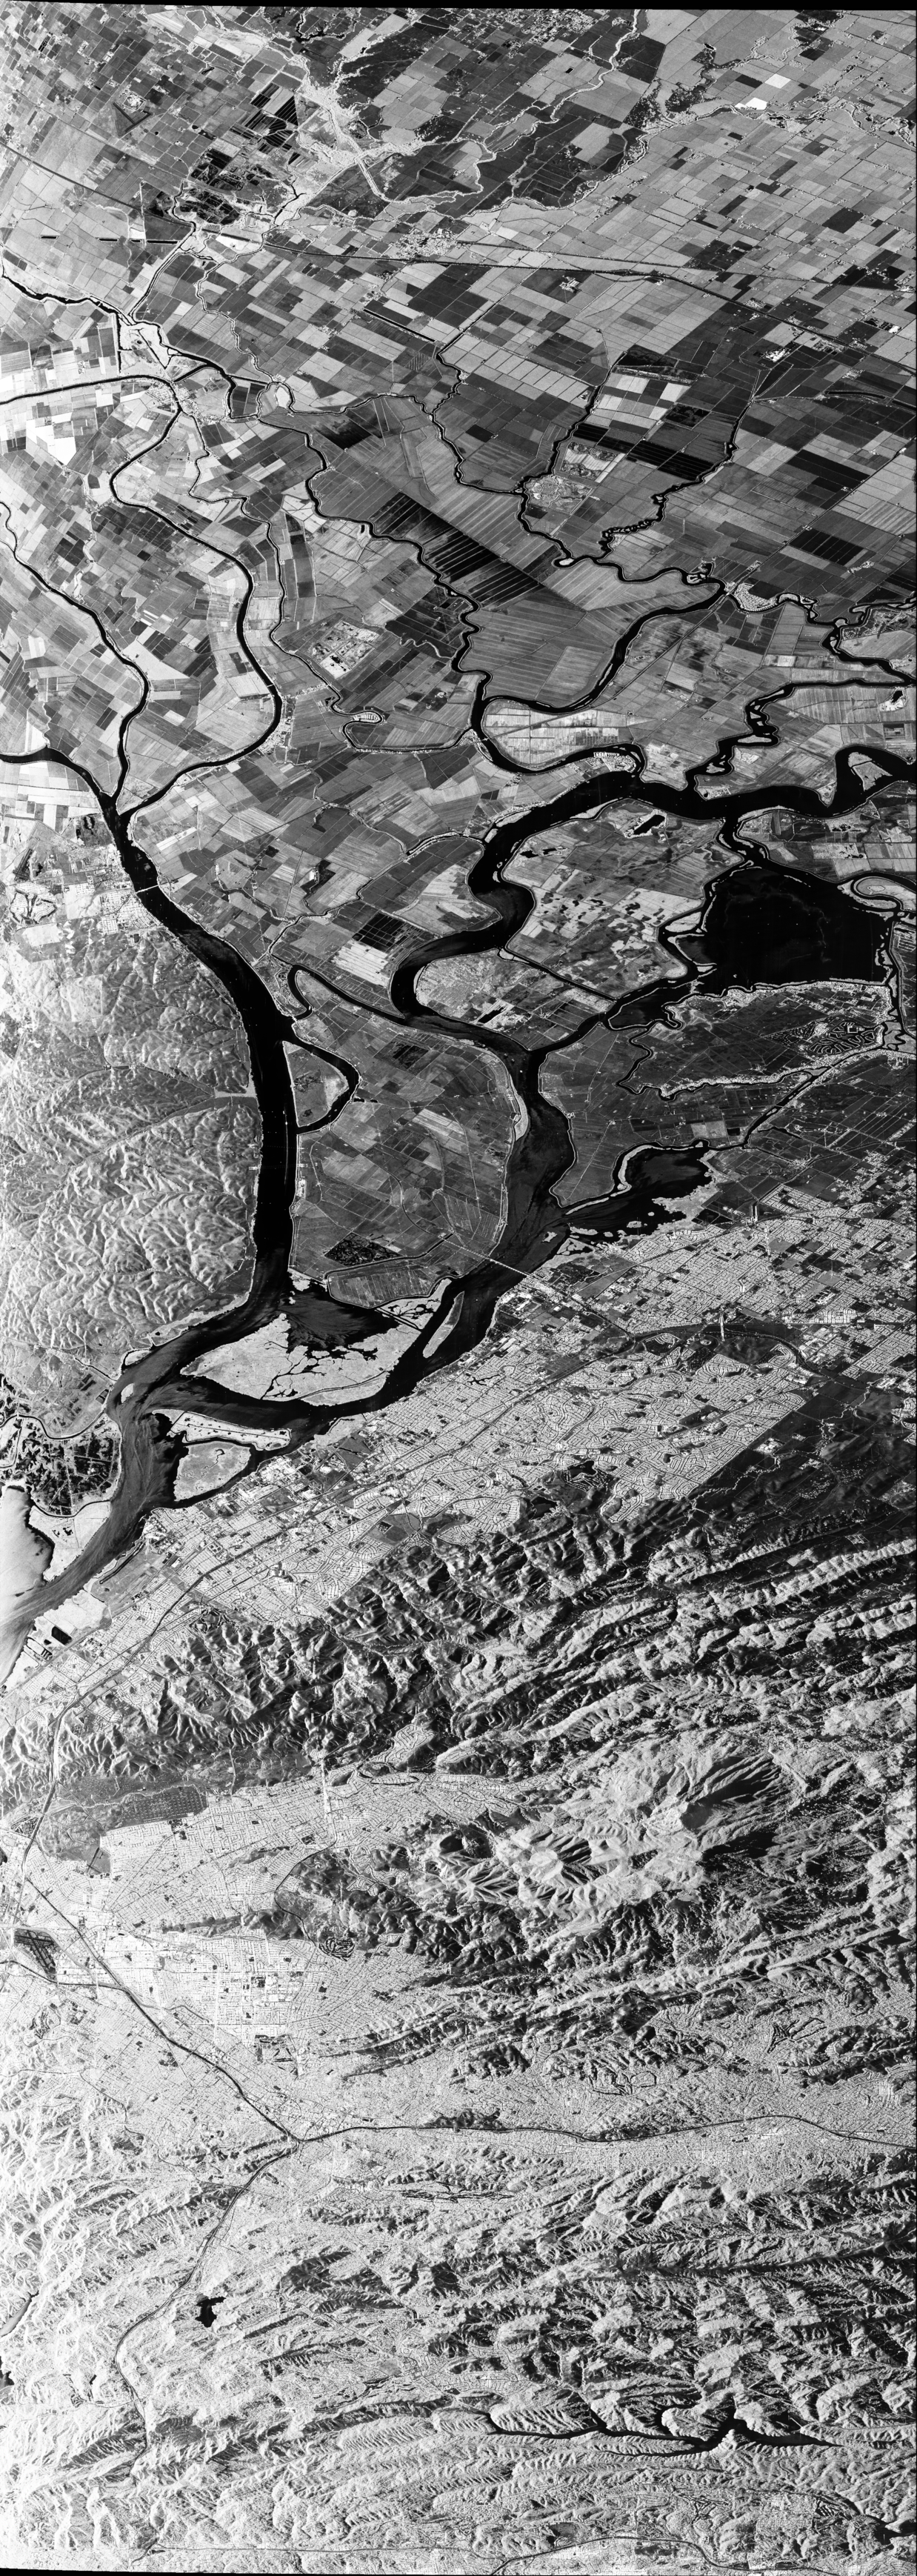
\includegraphics[width=.3\linewidth]{Images/Pauli_Sa.png}}
	\subcaptionbox{expressa a intensidade da energia presente no componente $S_{b}$ associados aos pixeis. Este  corresponde ao mecanismo de espalhamento de um diedro orientado à $0^\circ$ "double or even-bounce scattering". \label{fig:Pauli_Sb}}{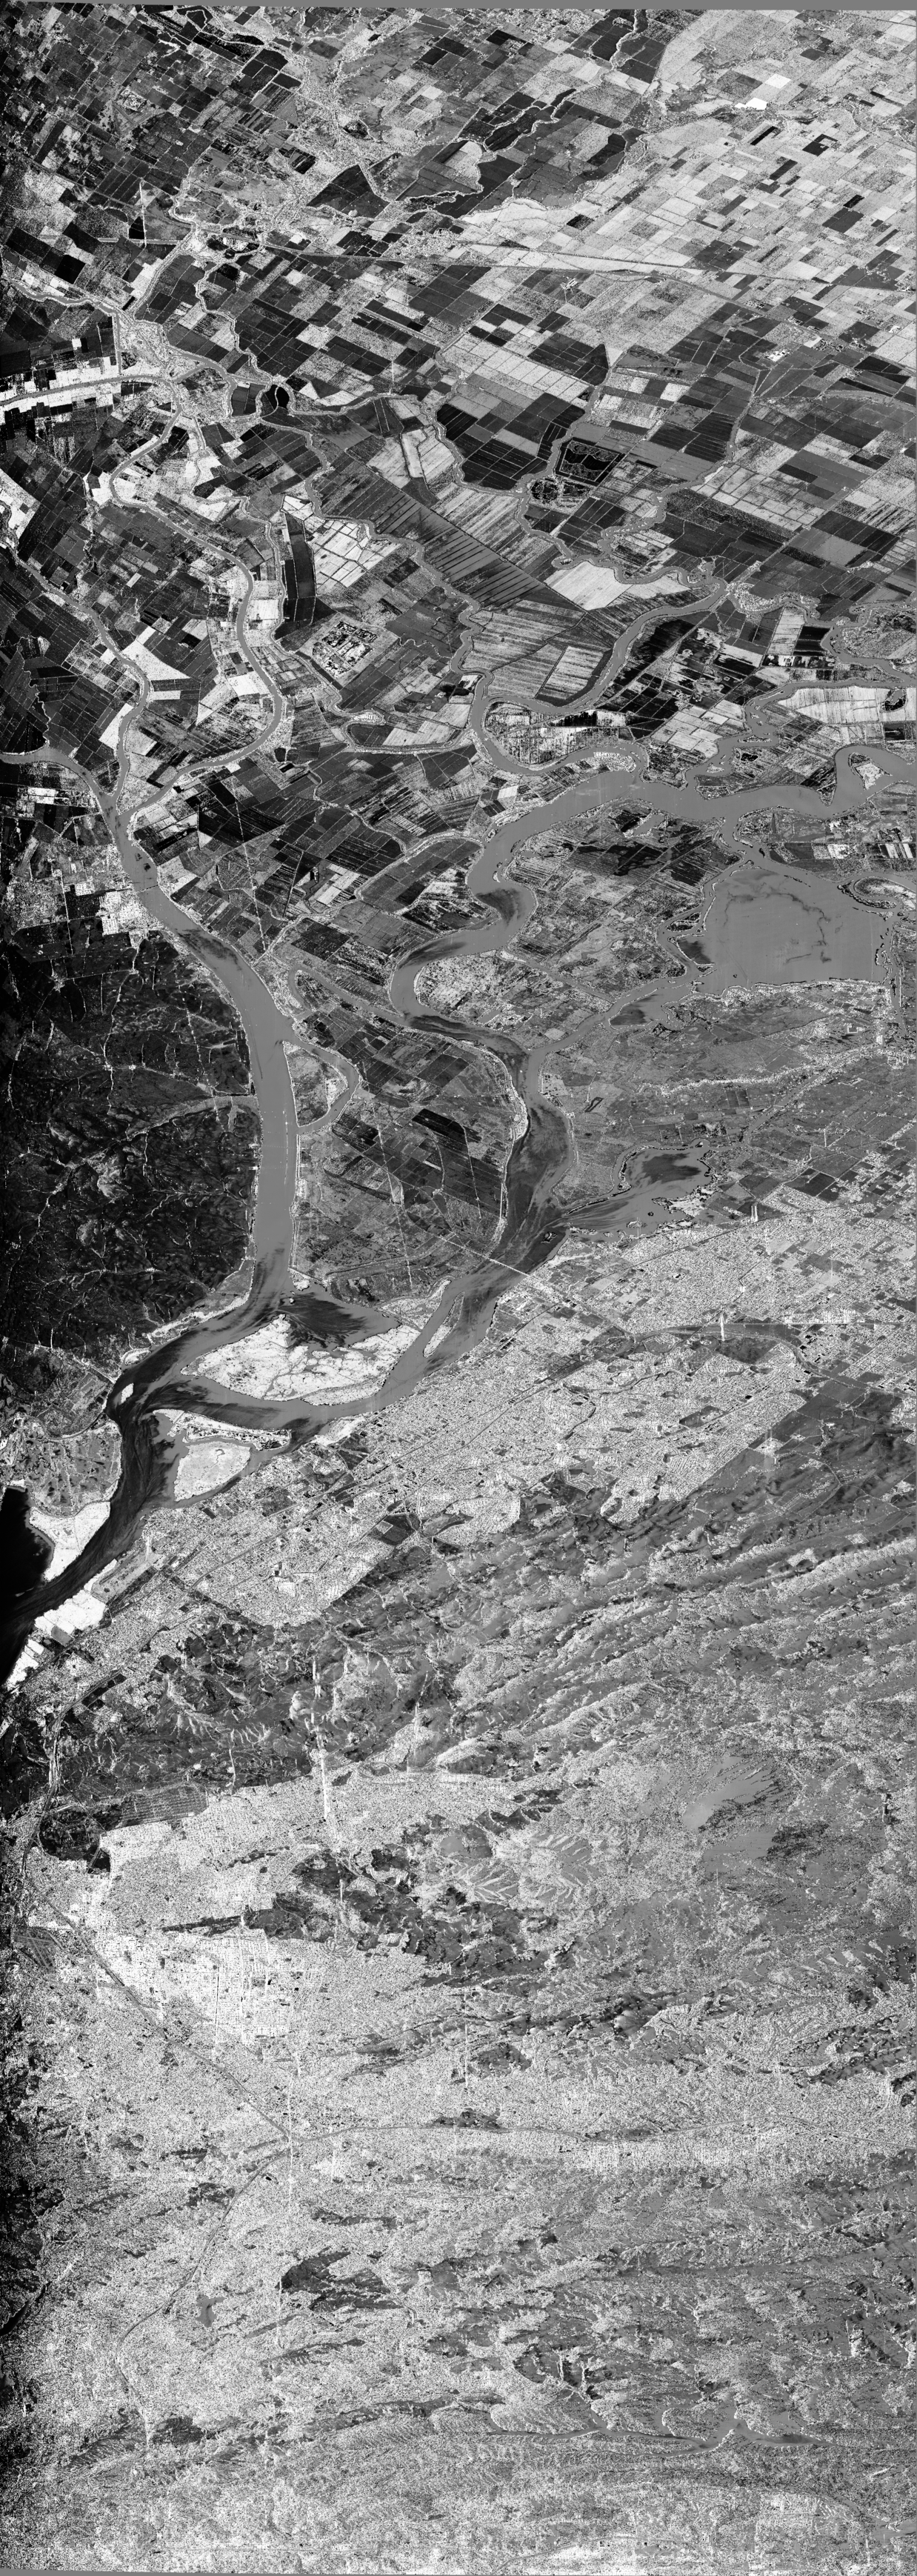
\includegraphics[width=.3\linewidth]{Images/Pauli_Sb.png}}
	\subcaptionbox{expressa a intensidade da energia presente no componente  $S_{c}$, que por sua vez, corresponde a contribuição do mecanismo de espalhamento de um diedro orientado à $45^\circ$ "double or even-bounce scattering".
	\label{fig:Pauli_Sc}}{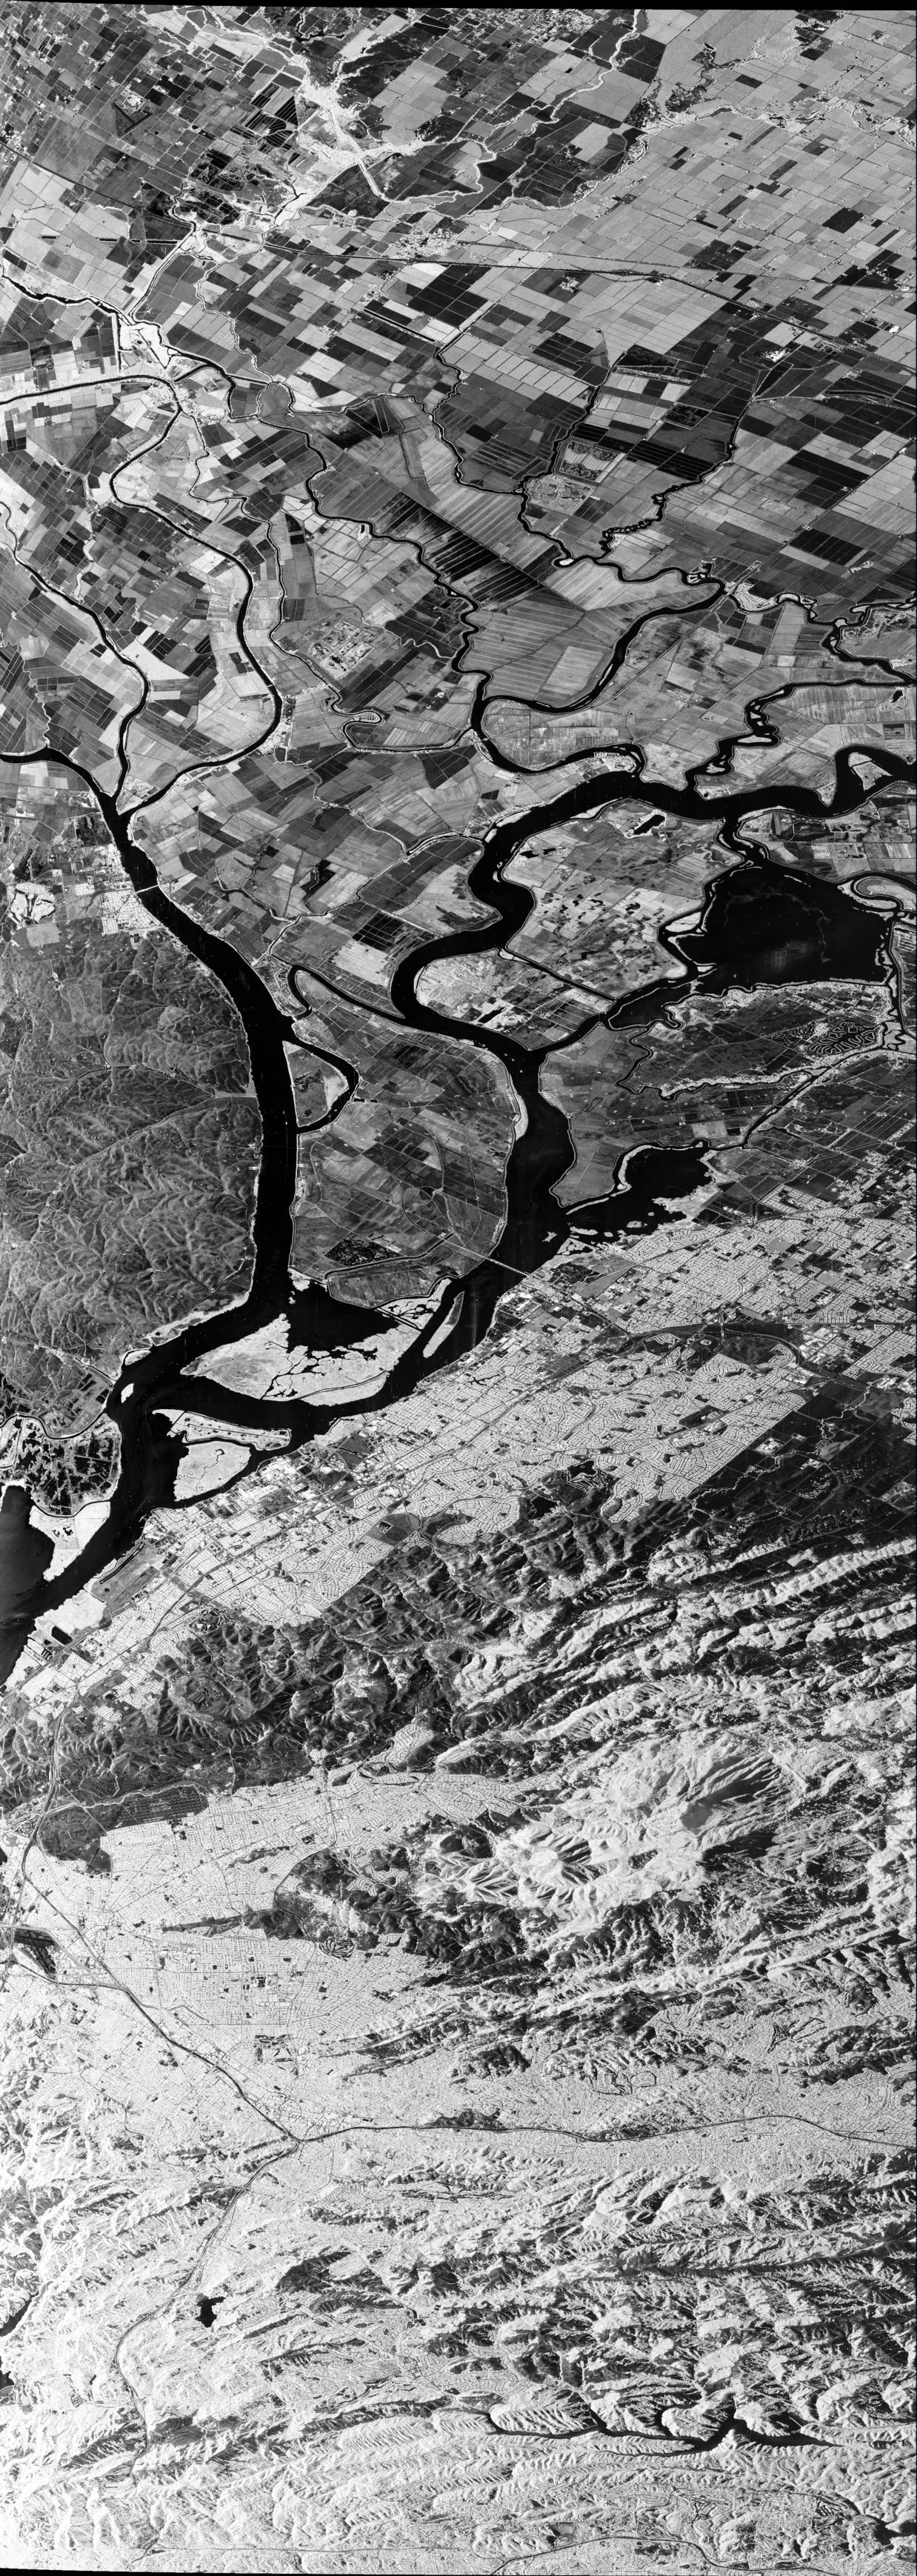
\includegraphics[width=.3\linewidth]{Images/Pauli_Sc.png}}
    \caption{Imagens dos três mecanismos de espalhamento.}
\end{figure}

\begin{figure}[H]
    \centering
    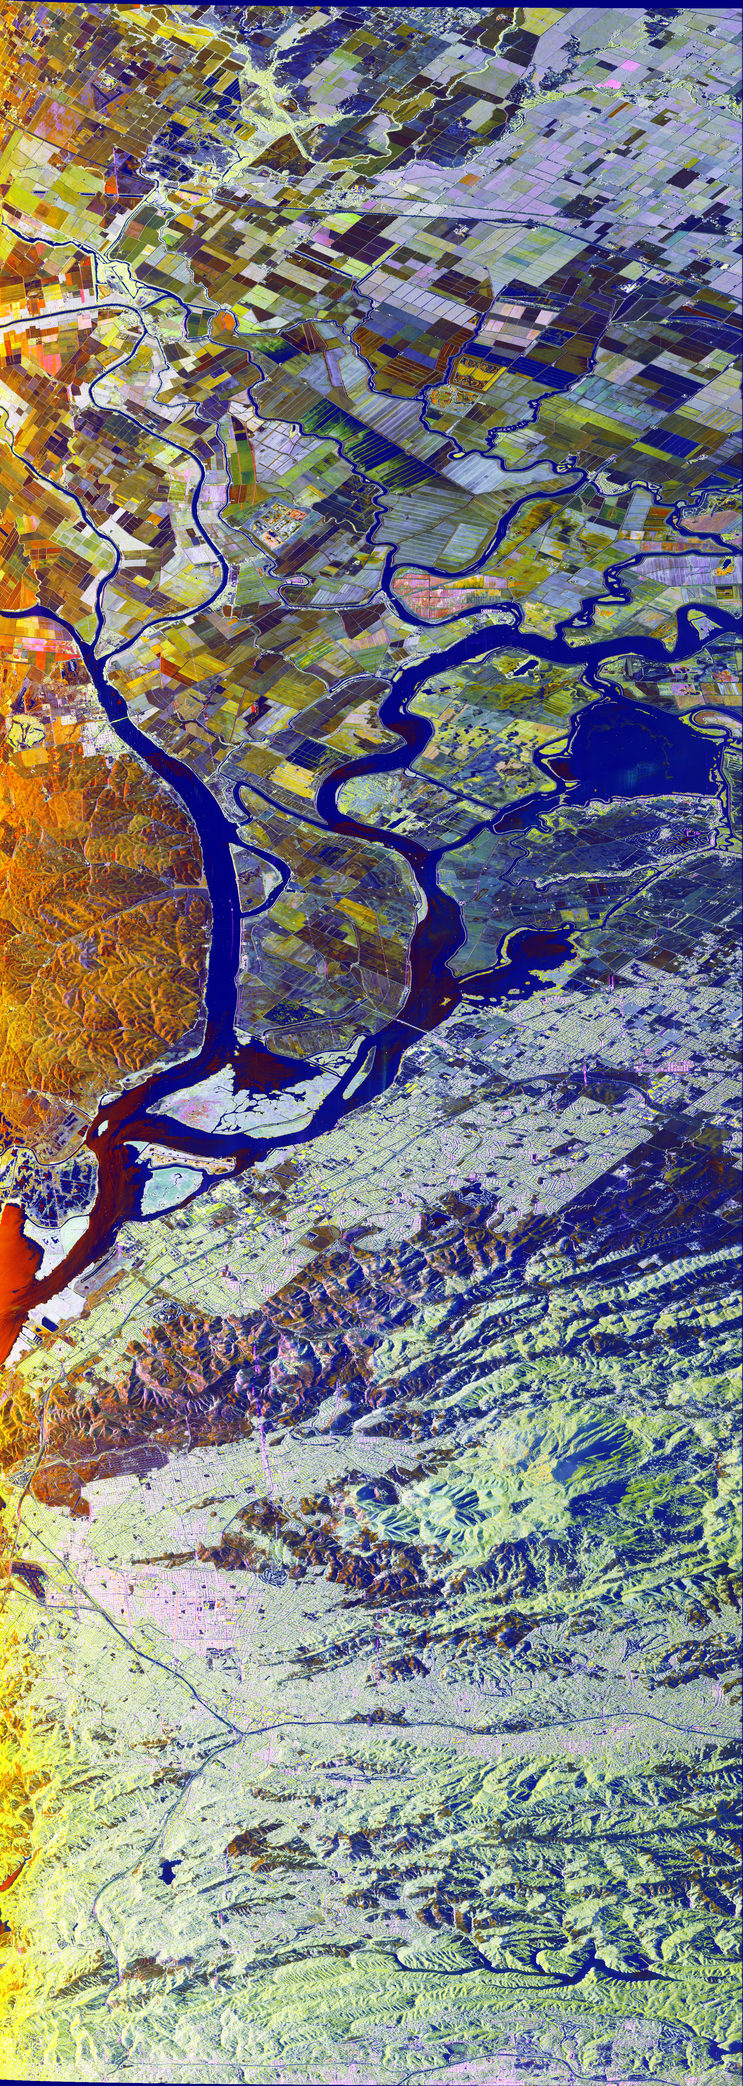
\includegraphics[width=.4\linewidth]{Images/Pauli.png}
    \caption{Imagem gerada depois da aplicação da decomposição de Pauli, que combina os três mecanismos de espalhamento. A tabela ~\ref{tab:code_color_pauli} mostra o esquema de codificação de cores.} 
    \label{fig:Pauli}
\end{figure}

\begin{table}[H]
    \centering
    \begin{tabular}{|c|c|c|}
         \hline
         Vetor & Mecanismo de espalhamento & Cor \\ \hline
         $S_{a}$ & $(S_{hh} + S_{hh}) \frac{1}{\sqrt{2}}$ & Vermelho \\ \hline
         $S_{b}$ & $(S_{hh} - S_{hh}) \frac{1}{\sqrt{2}}$ & Verde \\ \hline
         S$_{c}$ & $(2S_{vh}) \frac{1}{\sqrt{2}}$ & Azul \\ \hline
    \end{tabular}
    \caption{Decomposição de Pauli codificado em canal RGB.}
    \label{tab:code_color_pauli}
\end{table}

\subsection{\textbf{Krogager}}

\begin{figure}[H]
	\subcaptionbox{representa a energia presente no componente $K_{d}$ que corresponde a contribuição da esfera. \label{fig:KrogagerK_{d}}}{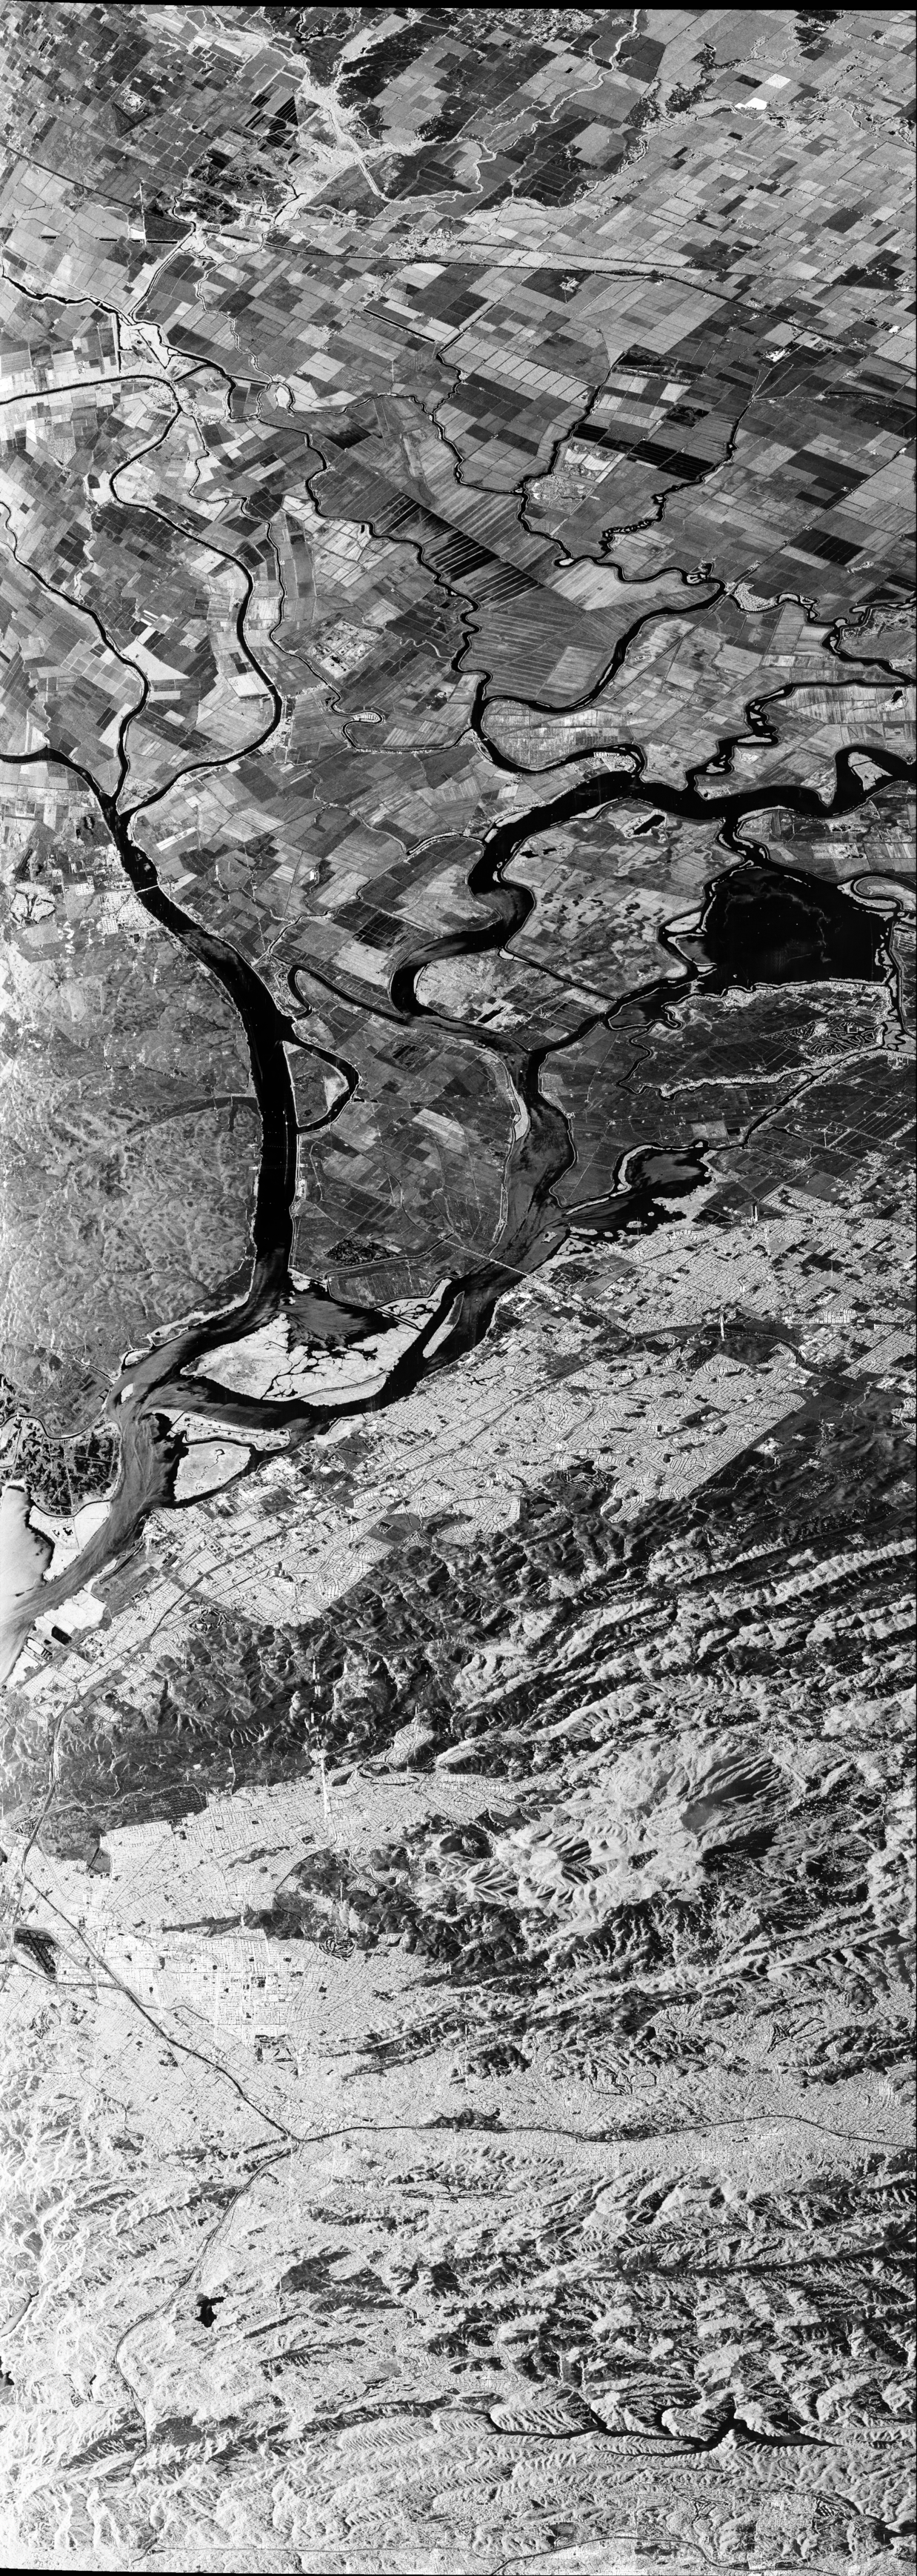
\includegraphics[width=.3\linewidth]{Images/KrogagerKd.png}}
	\subcaptionbox{representa a energia presente no componente $K_{h}$ que corresponde a contribuição de um biplano. \label{fig:KrogagerK_{h}}}{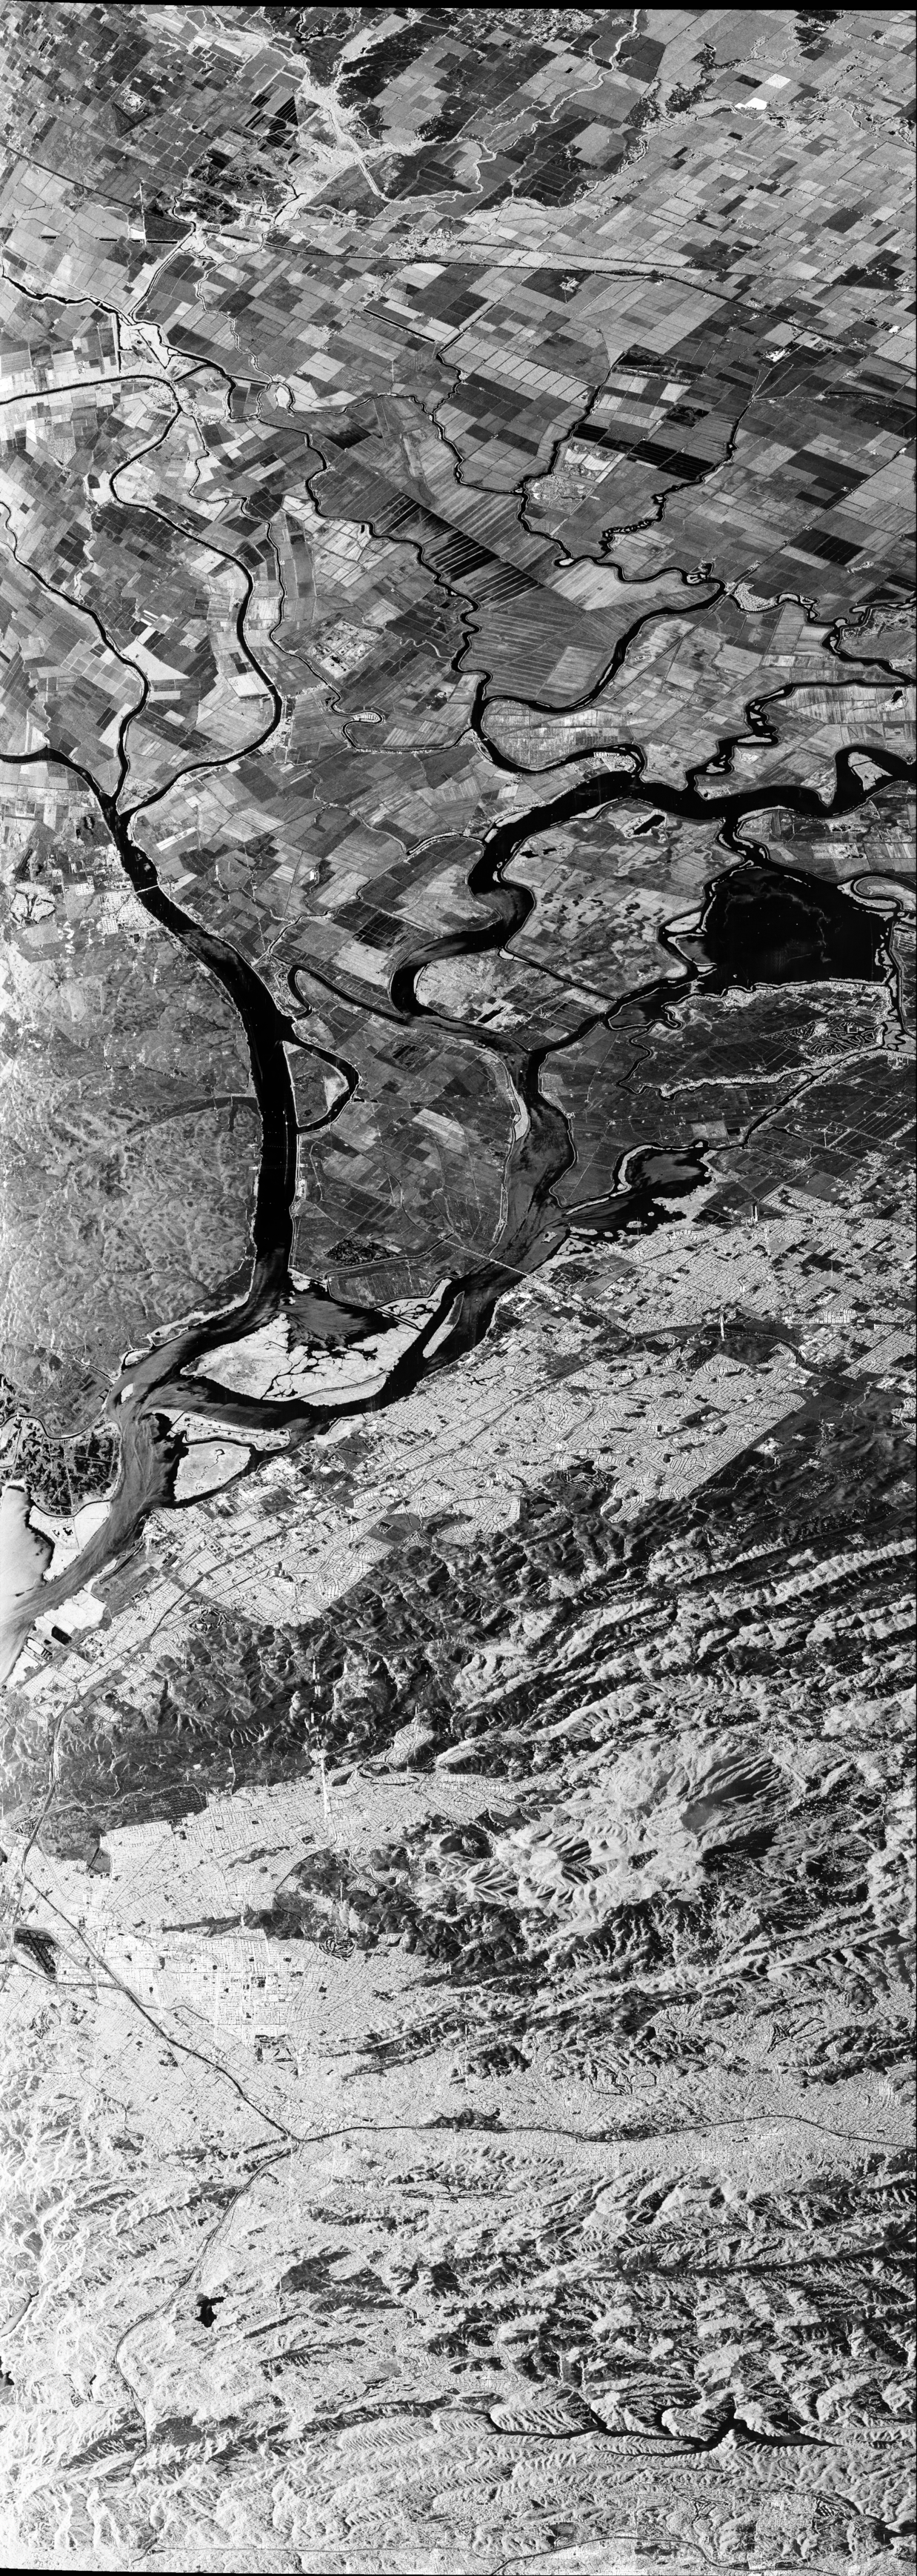
\includegraphics[width=.3\linewidth]{Images/KrogagerKh.png}}
	\subcaptionbox{representa a energia presente no componente $K_{s}$ que corresponde a contribuição de uma espiral.
	\label{fig:KrogagerK_{s}}}{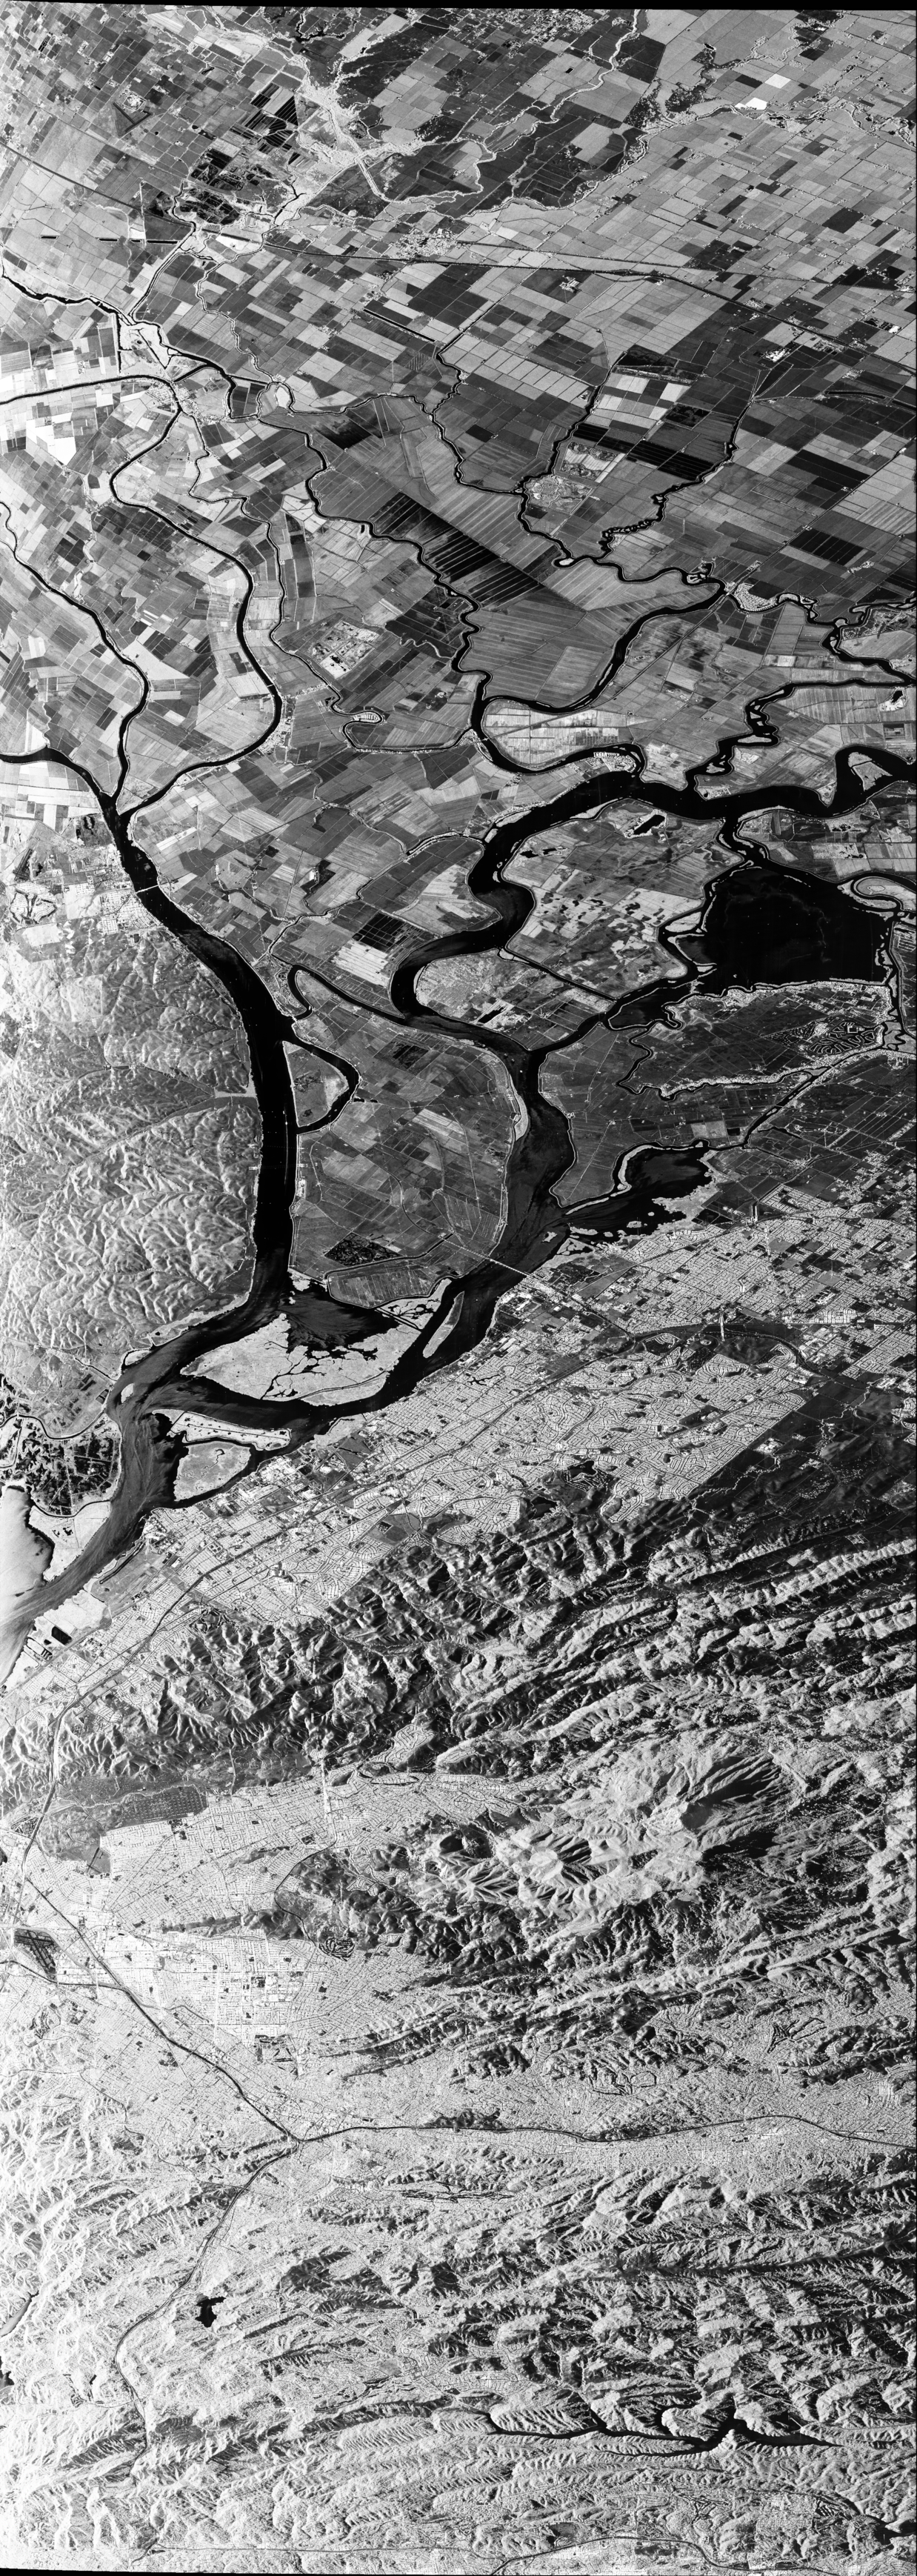
\includegraphics[width=.3\linewidth]{Images/KrogagerKs.png}}
    \caption{Imagens separadas em três mecanismos de espalhamento.}
\end{figure}

\begin{figure}[H]
    \centering
    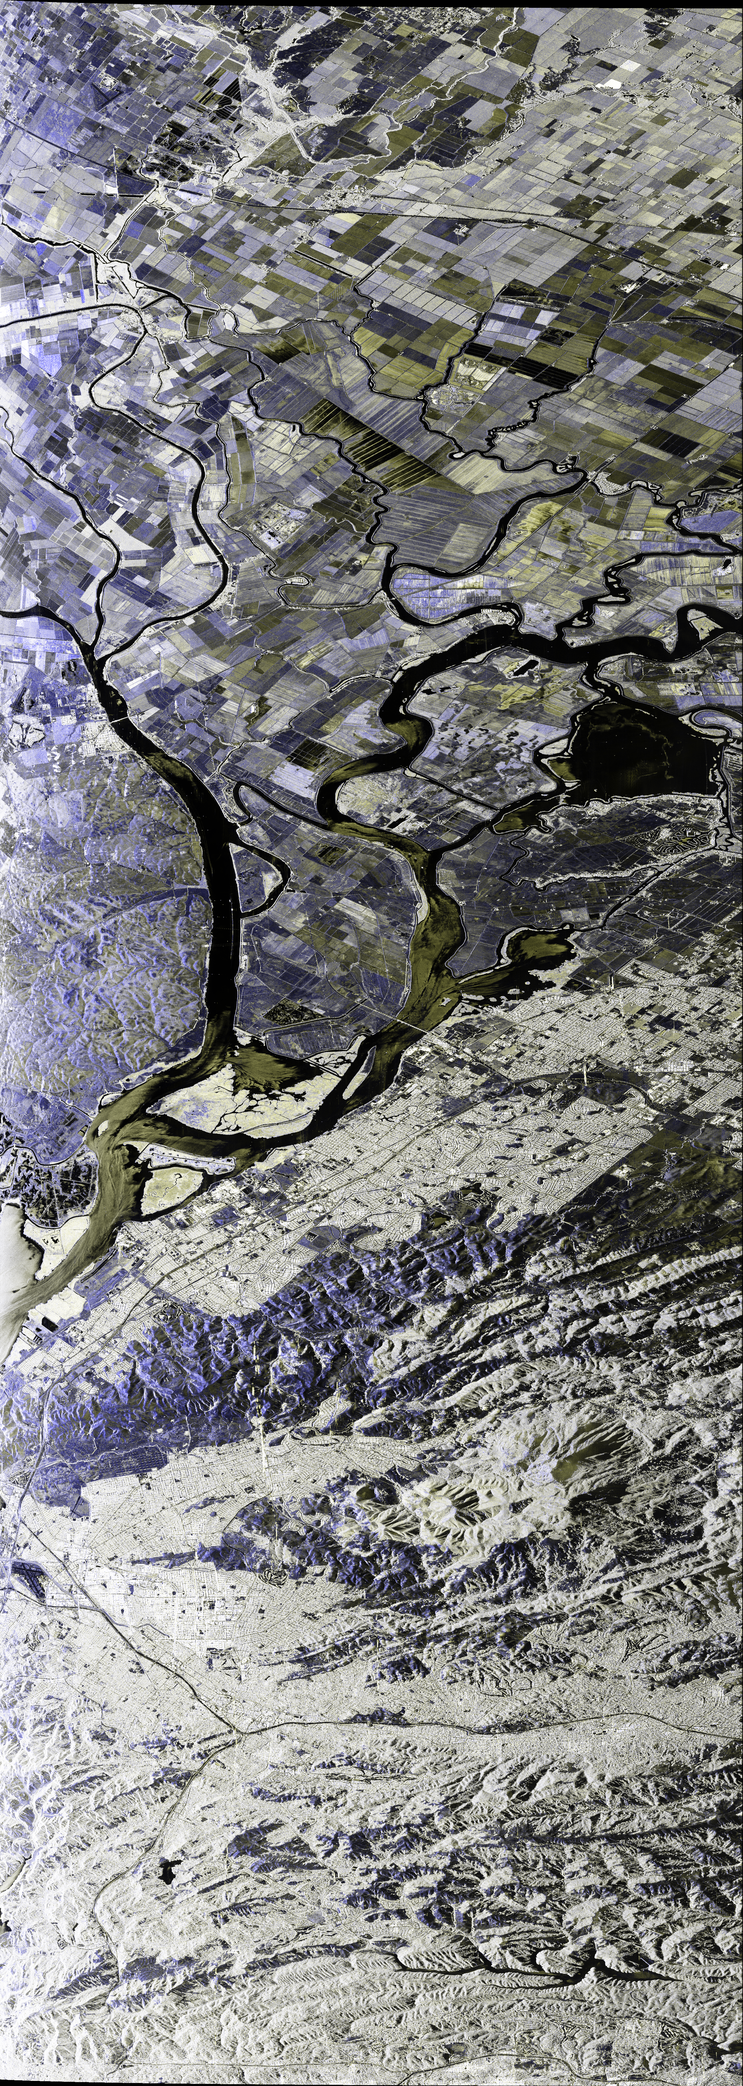
\includegraphics[width=.4\linewidth]{Images/Krogager.png}
    \caption{Imagem gerada depois da aplicação da decomposição de Krogager, que combina os três mecanismos de espalhamento. A tabela \ref{tab:code_color_krogager} mostra o esquema de codificação de cores.} 
    \label{fig:Krogager}
\end{figure}

\begin{table}[H]
    \centering
    \begin{tabular}{|c|c|c|}
         \hline
         Vetor & Mecanismo de espalhamento & Cor \\ \hline
         $K_{d}$ & $\sqrt{B_{0}-F}$ & Vermelho \\ \hline
         $K_{h}$ & $\sqrt{B_{0}+F} - \sqrt{B_{0}-F}$ & Verde \\ \hline
         $K_{s}$ & $\sqrt{A_{0}}$ & Azul \\ \hline
    \end{tabular}
    \caption{Decomposição de Krogager codificado em canal RGB.}
    \label{tab:code_color_krogager}
\end{table}

\subsection{\textbf{Hyunem}}

\begin{figure}[H]
	\subcaptionbox{representa a energia presente no componente $T_{22T}$. \label{fig:Hyunem_22T}}{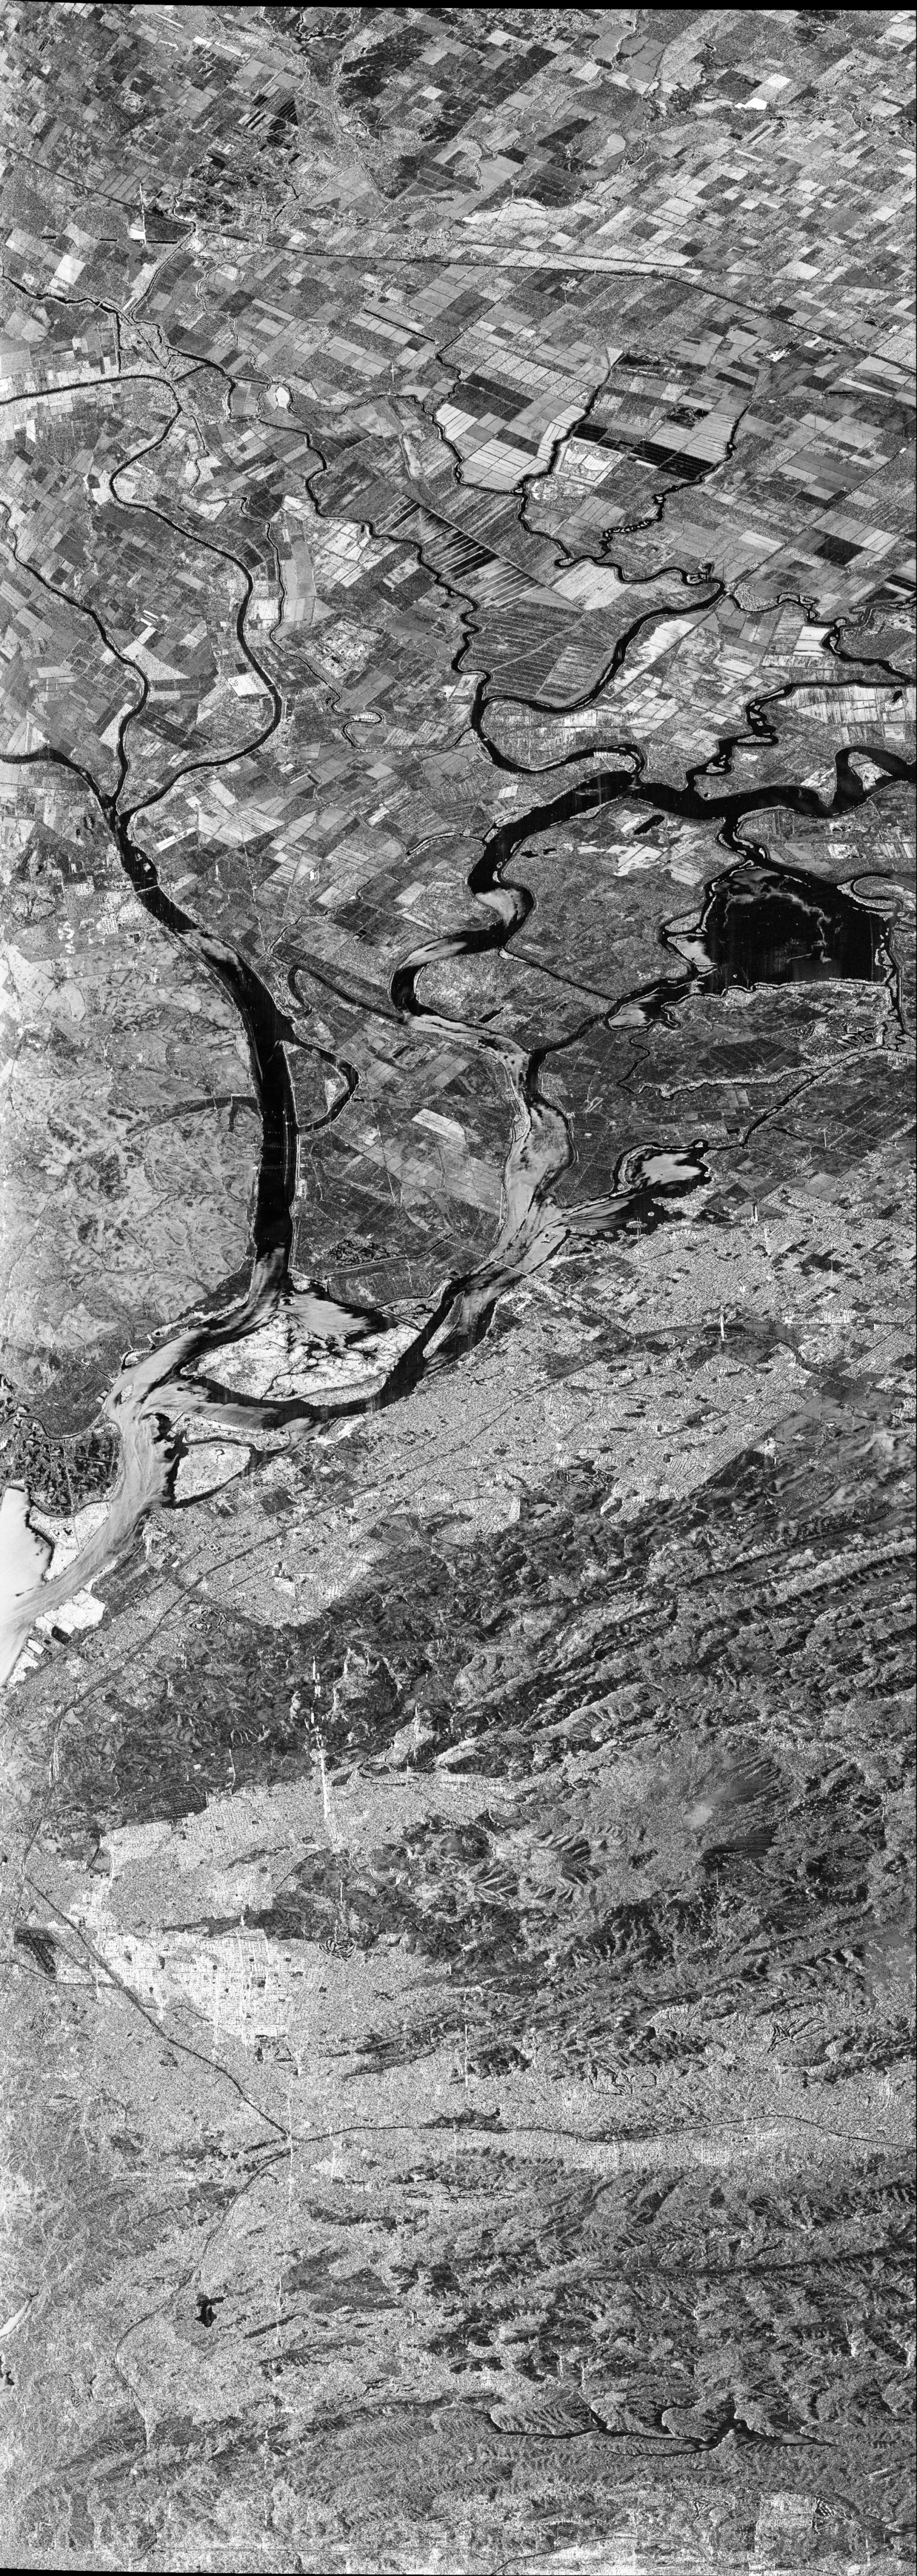
\includegraphics[width=.3\linewidth]{Images/Hyunen_22T.png}}
	\subcaptionbox{representa a energia presente no componente $T_{33T}$. \label{fig:Hyunem_33T}}{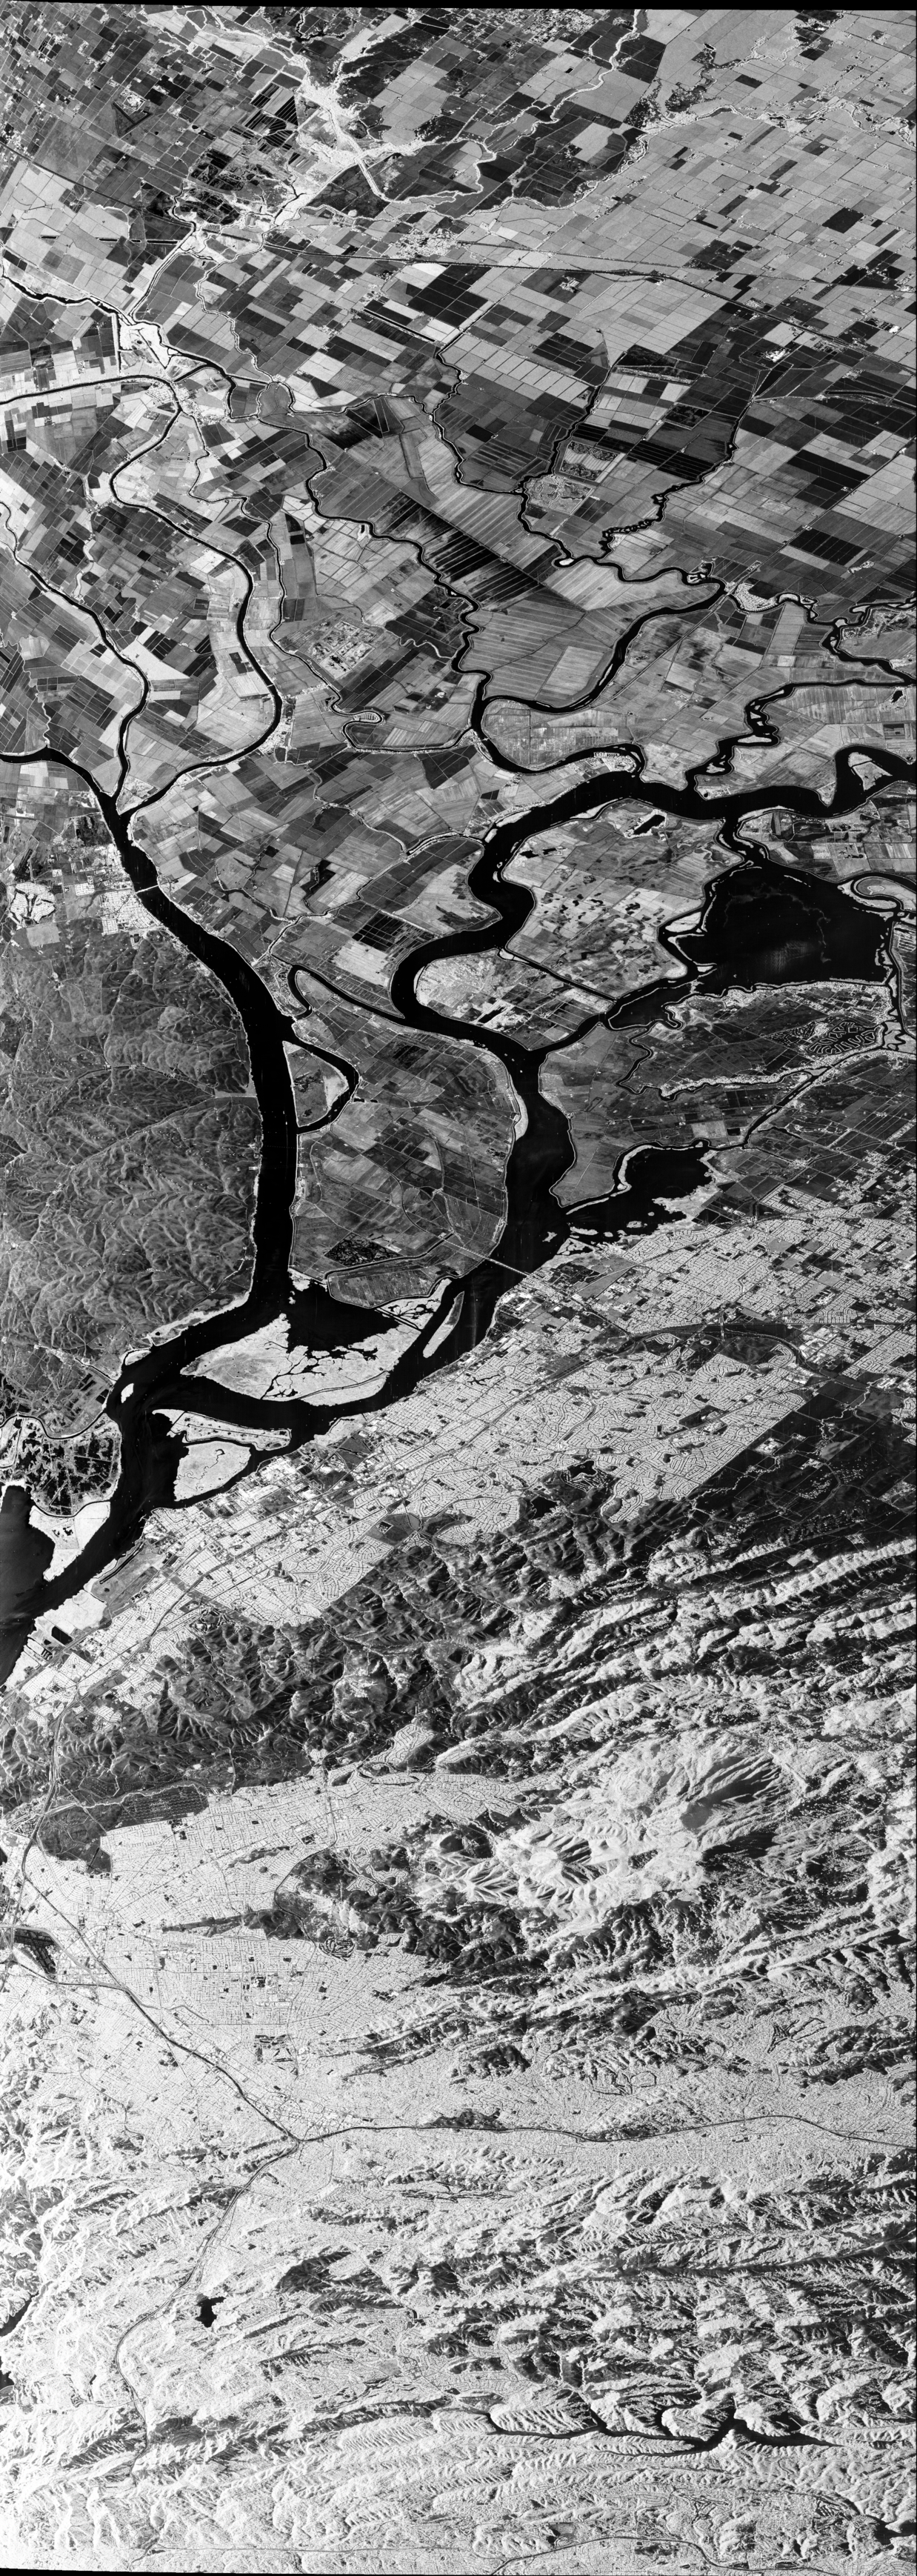
\includegraphics[width=.3\linewidth]{Images/Hyunen_33T.png}}
	\subcaptionbox{representa a energia presente no componente $T_{11T}$. \label{fig:Hyunem_11T}}{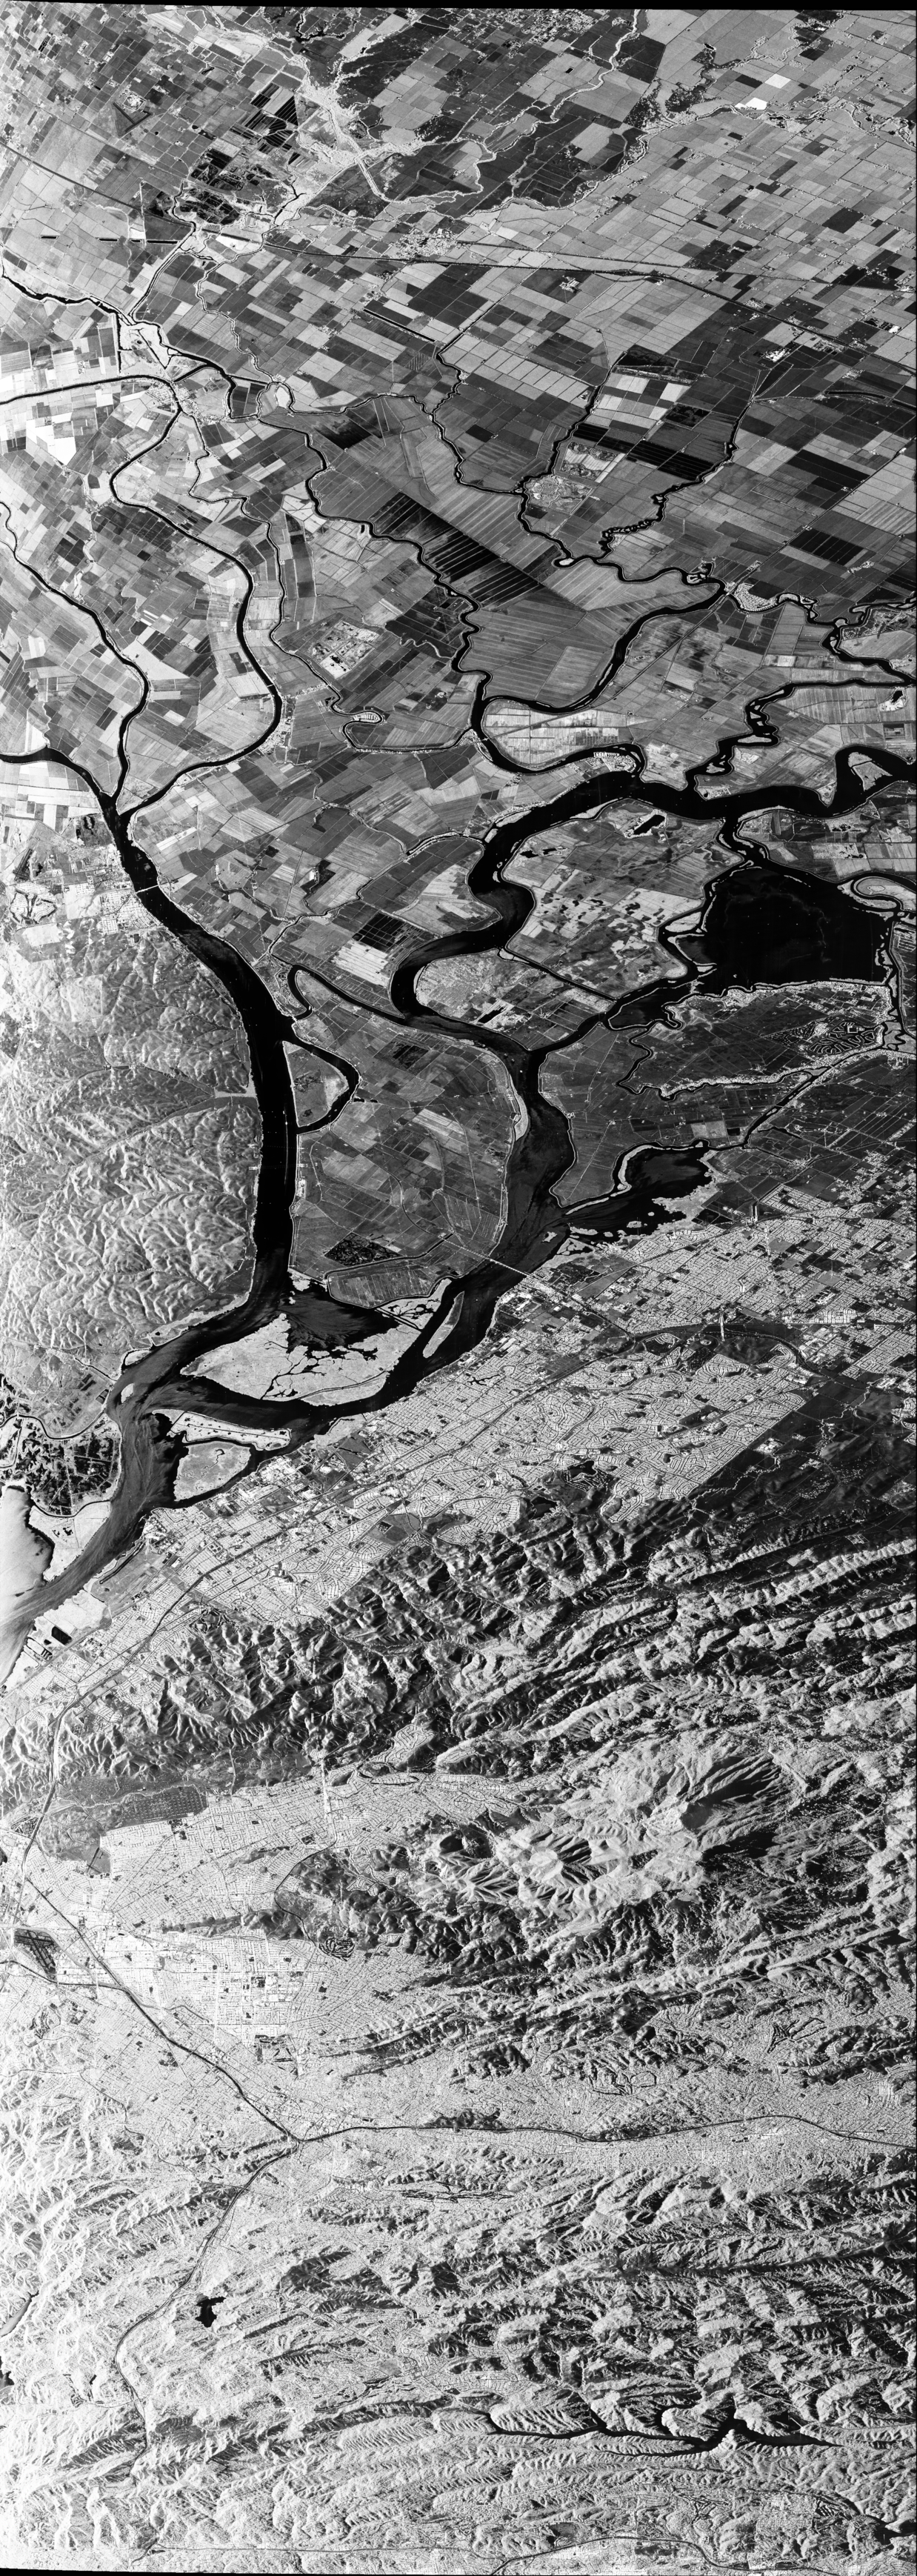
\includegraphics[width=.3\linewidth]{Images/Hyunen_11T.png}}
    \caption{As imagens dos três componentes geradores.}
\end{figure}

\begin{figure}[H]
    \centering
    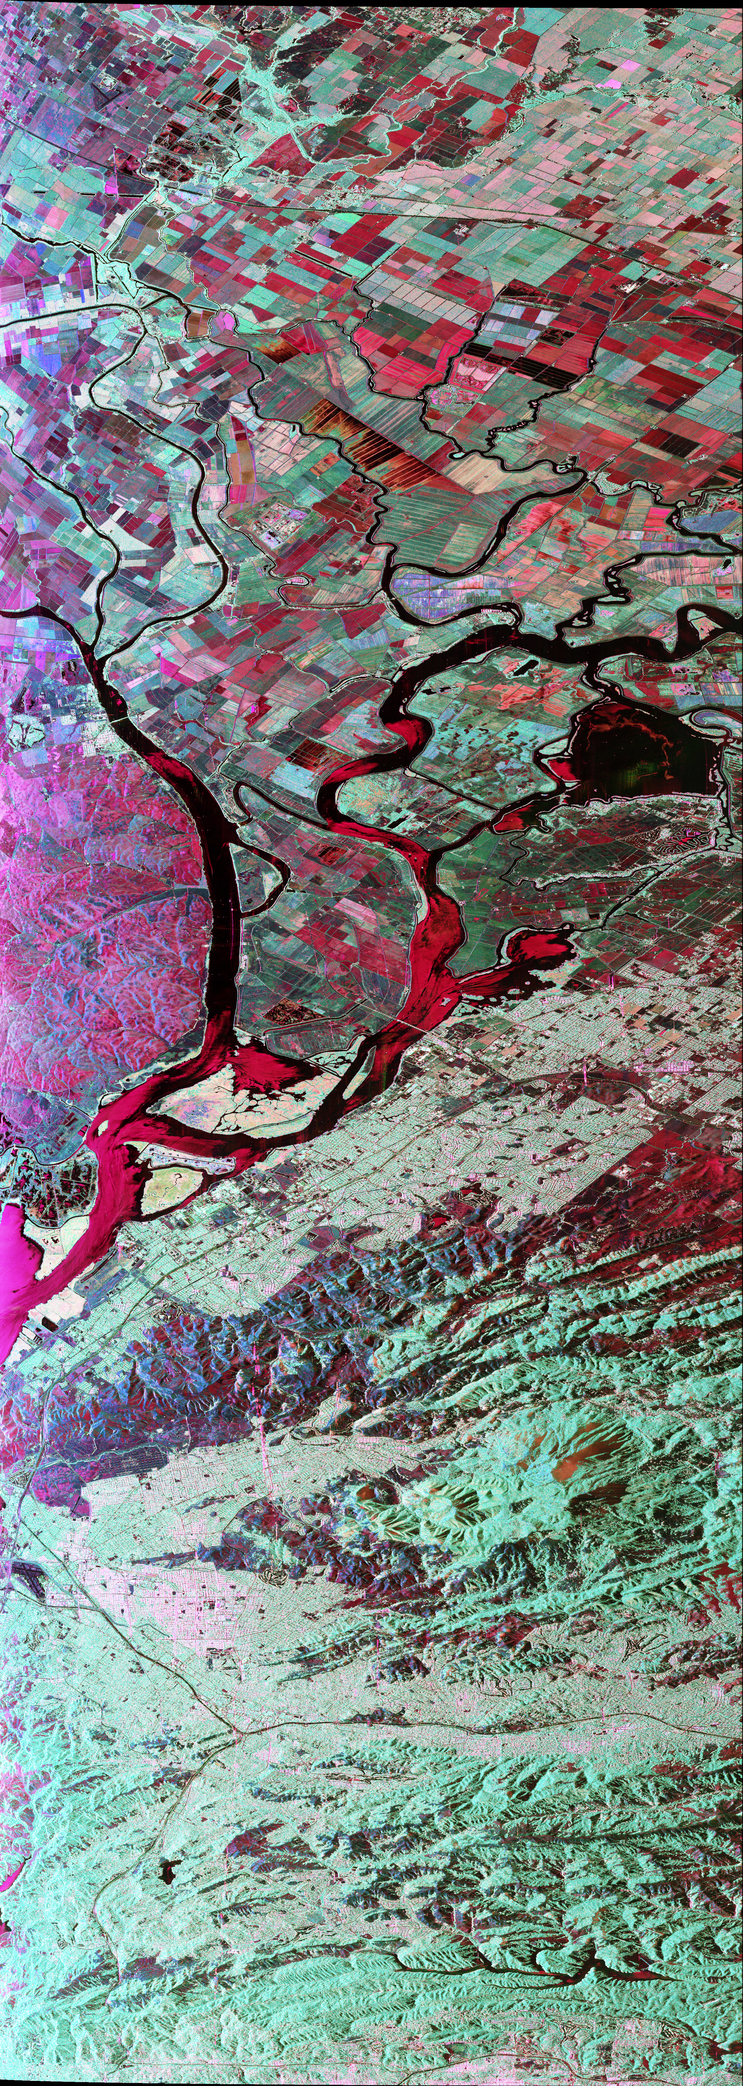
\includegraphics[width=.4\linewidth]{Images/Hyunen.png}
    \caption{A combinação dos três componentes geradores que tratem dos alvos únicos "alvos puros". A Tabela \ref{tab:code_color_hyunem} mostra o esquema de codificação de cores.}
    \label{fig:Hyunem}
\end{figure}

\begin{table}[H]
    \centering
    \begin{tabular}{|c|c|c|}
         \hline
         Vetor & Mecanismo de espalhamento & Cor \\ \hline
         $T_{22T}$ & $B_{0T} + B$ & Vermelho \\ \hline
         $T_{33T}$ & $B_{0T} - B_{T}$ & Verde \\ \hline
         $T_{11T}$ & $\langle2A_{0}\rangle$ & Azul \\ \hline
    \end{tabular}
    \caption{Decomposição de Hyunem codificado em canal RGB.}
    \label{tab:code_color_hyunem}
\end{table}


\subsection{\textbf{Barnes-Holmes}}

\begin{figure}[H]
	\subcaptionbox{representa a energia presente no componente $T_{22T}$. \label{fig:Barnes_22T}}{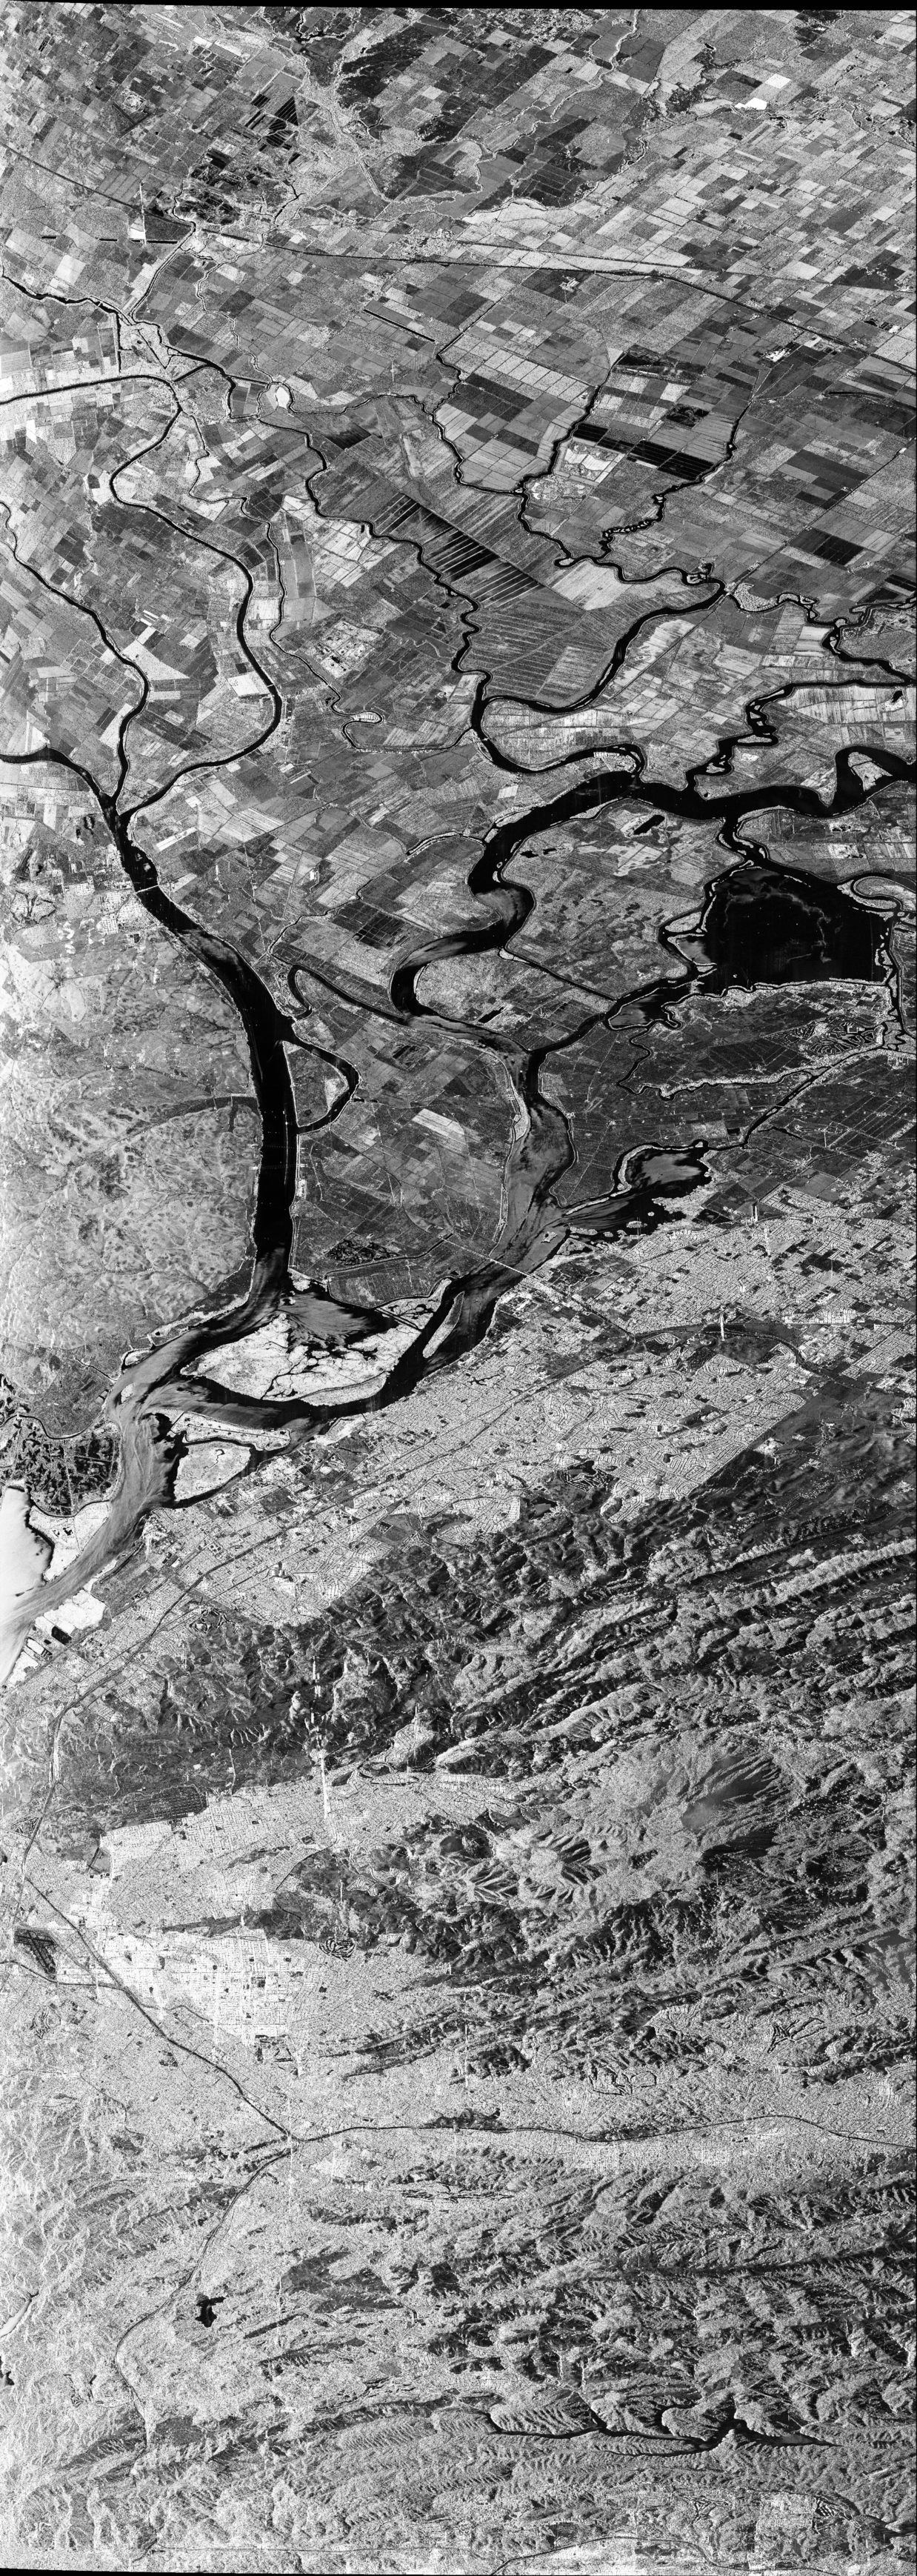
\includegraphics[width=.3\linewidth]{Images/Holmes_22T.png}}
	\subcaptionbox{representa a energia presente no componente $T_{33T}$. \label{fig:Barnes_33T}}{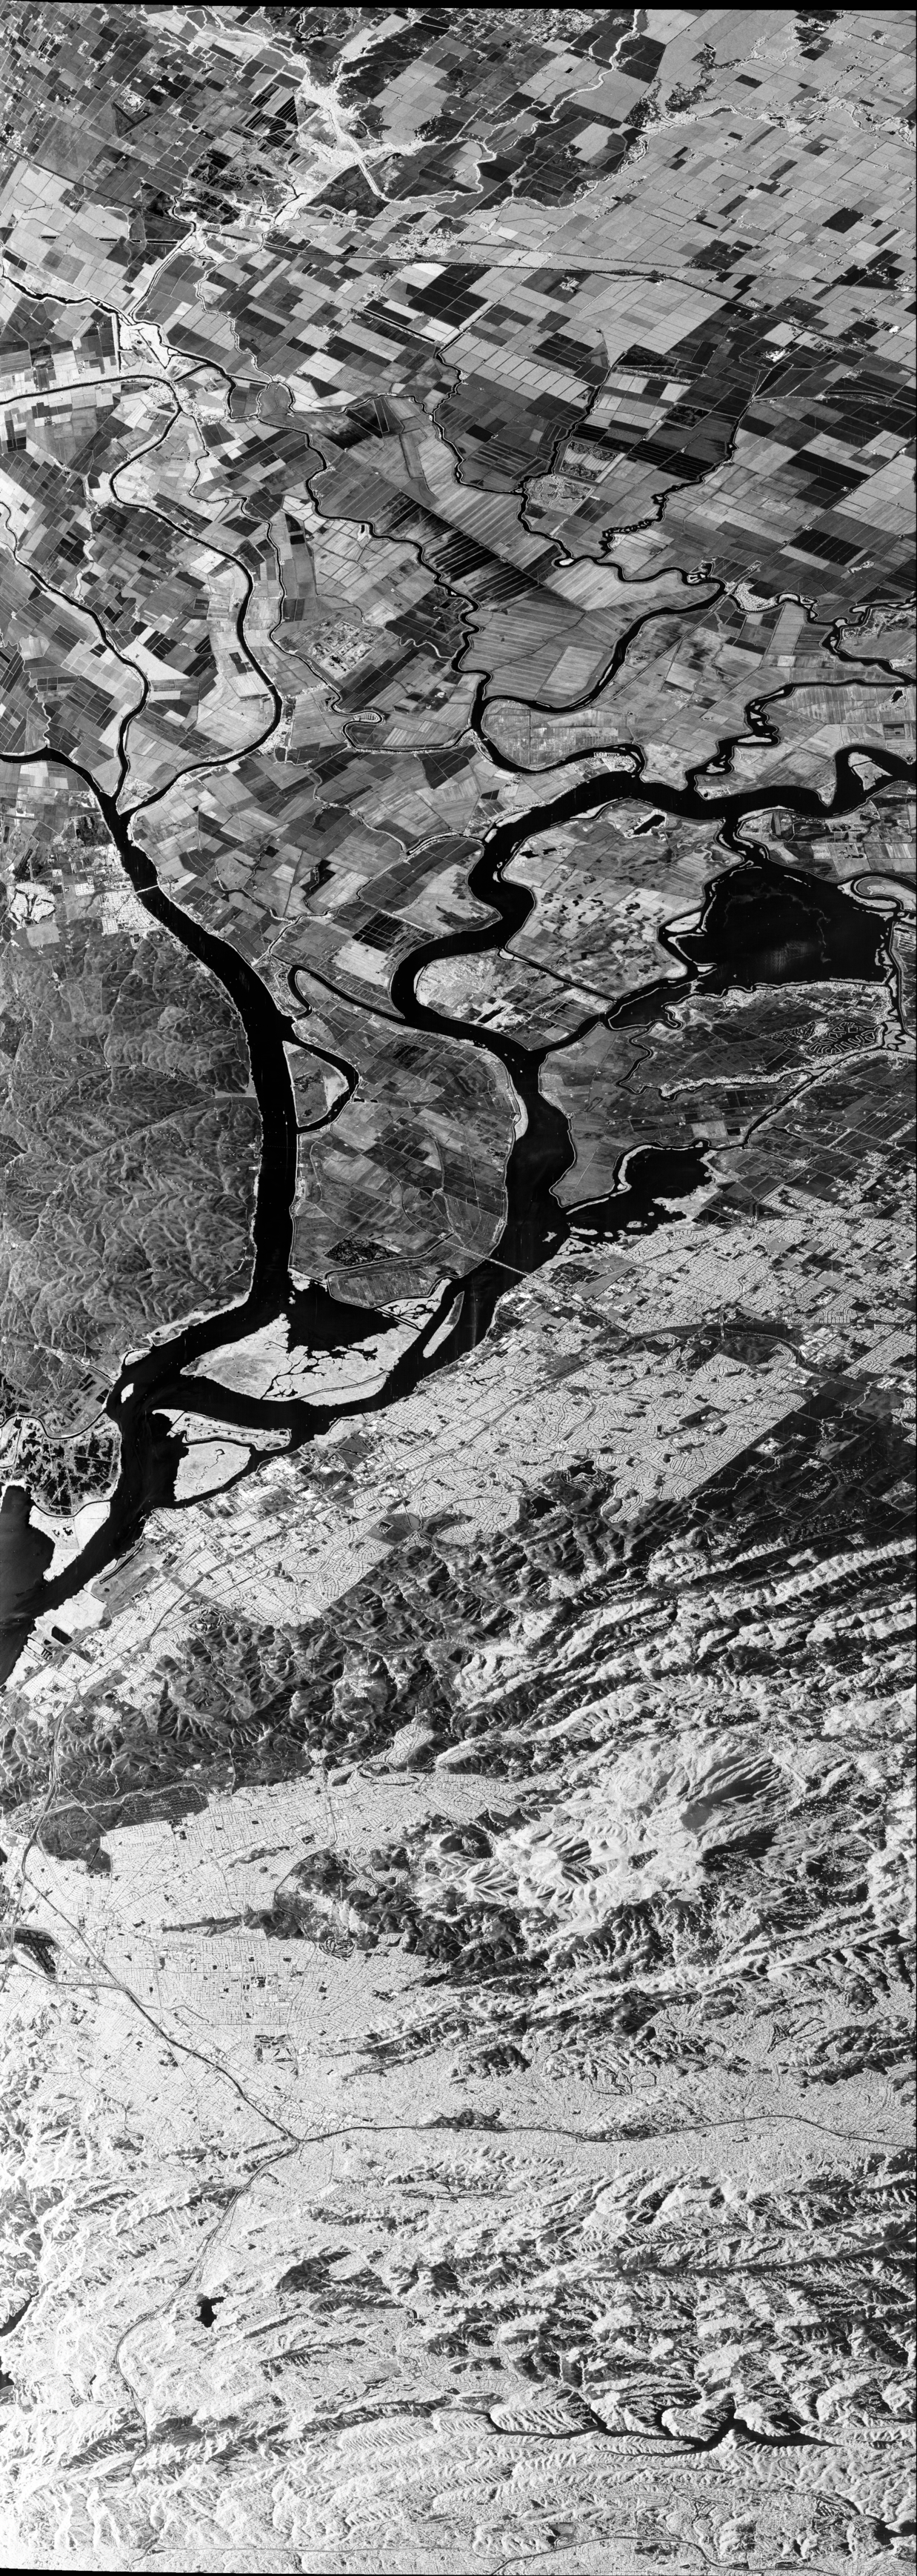
\includegraphics[width=.3\linewidth]{Images/Holmes_33T.png}}
	\subcaptionbox{representa a energia presente no componente $T_{11T}$. \label{fig:Barnes_11T}}{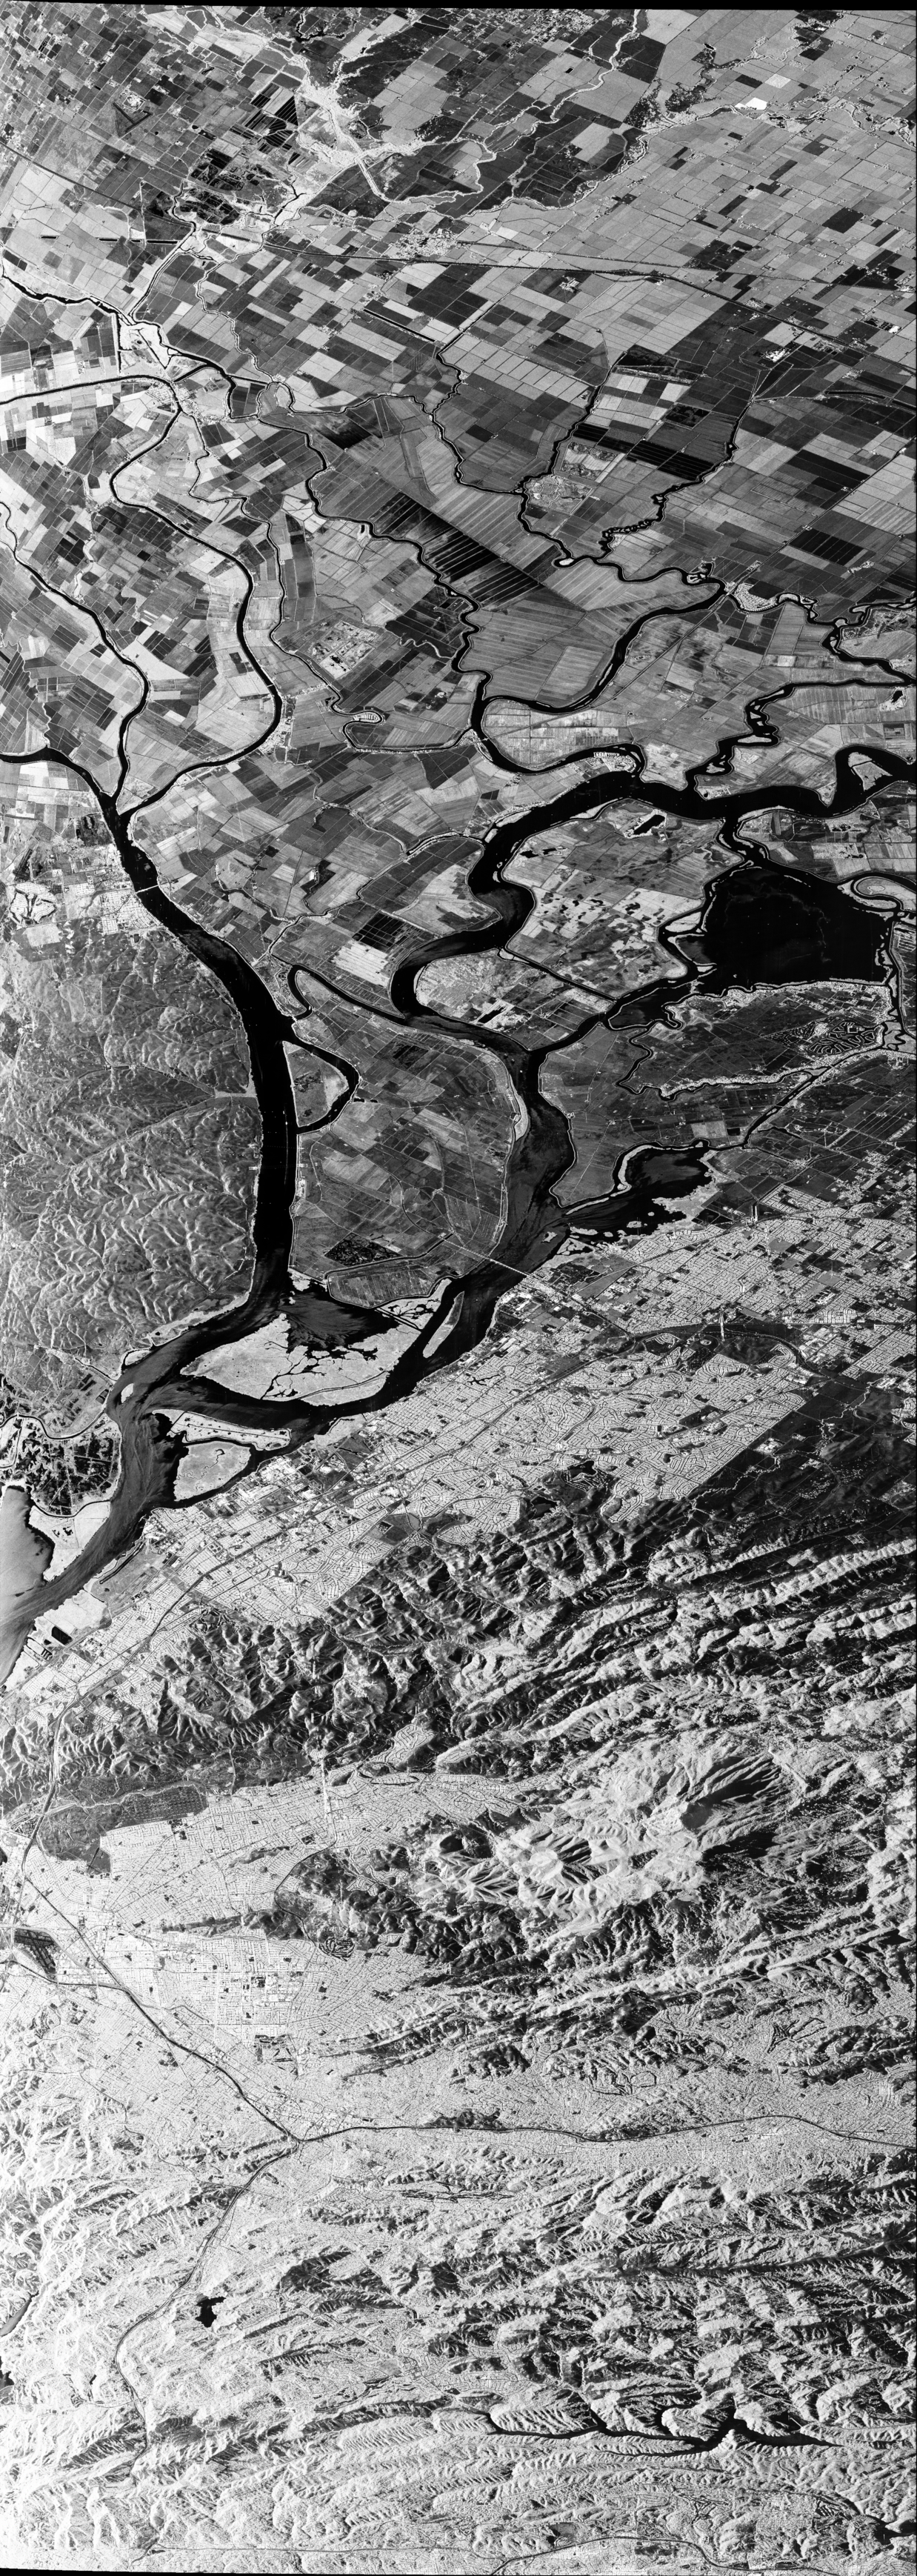
\includegraphics[width=.3\linewidth]{Images/Holmes_11T.png}}
    \caption{As imagens dos três componentes geradores.}
\end{figure}

\begin{figure}[H]
    \centering
    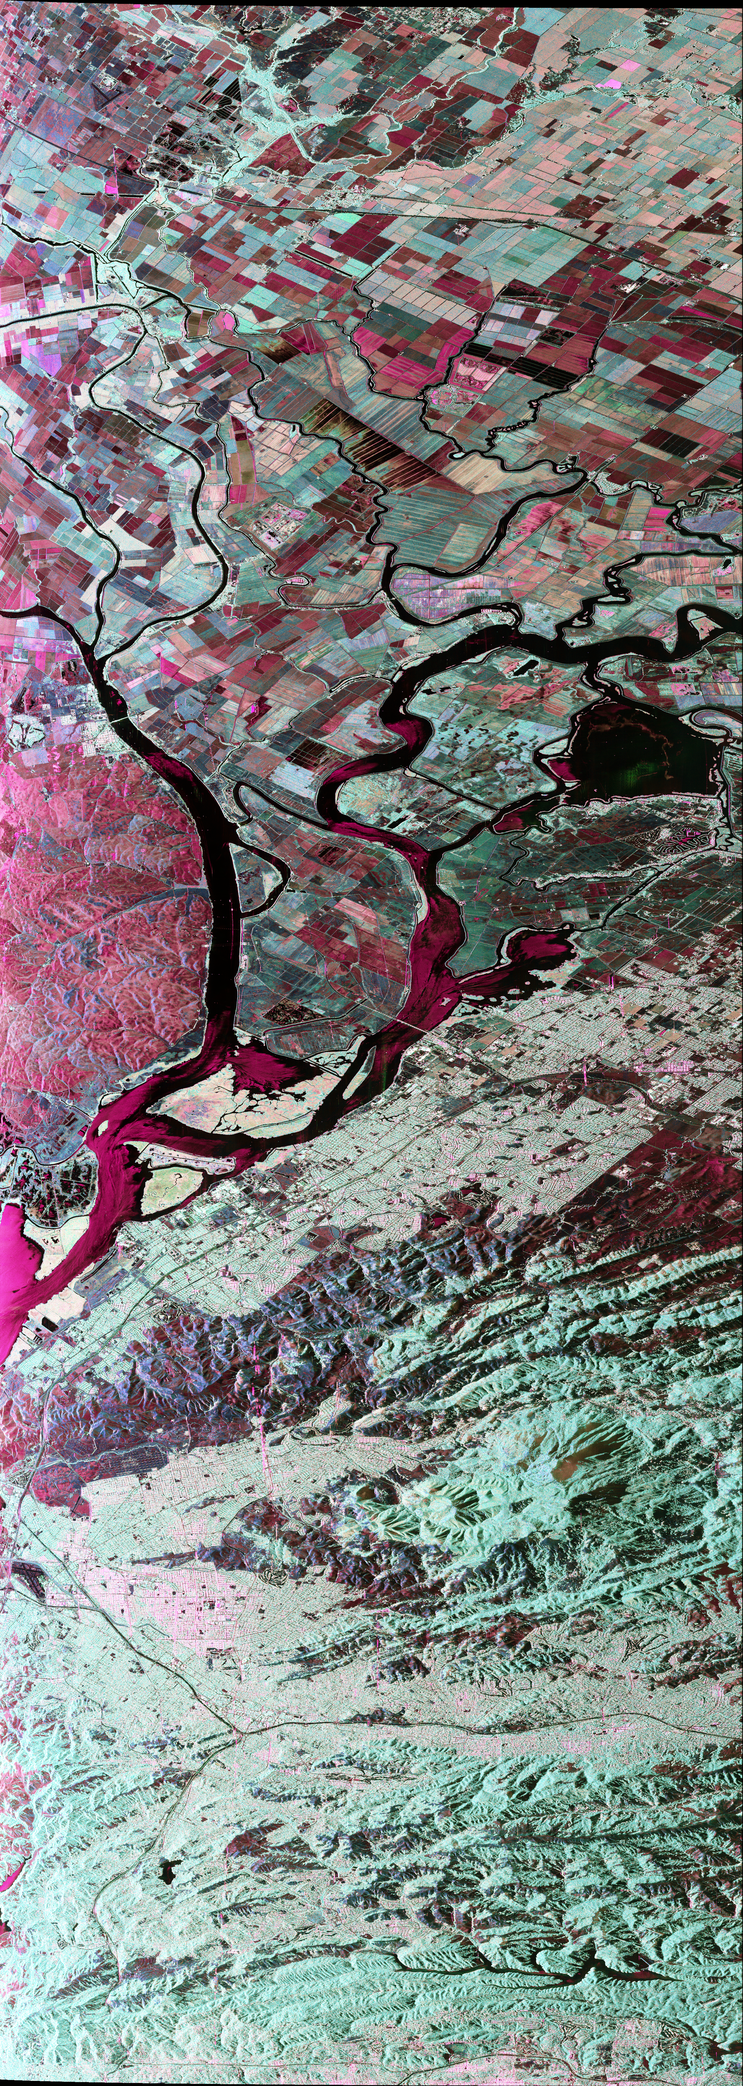
\includegraphics[width=.4\linewidth]{Images/Holmes.png}
    \caption{A combinação dos três componentes geradores que tratem dos alvos únicos "alvos puros". A Tabela \ref{tab:code_color_Barnes} mostra o esquema de codificação de cores.}
    \label{fig:Barnes}
\end{figure}

\begin{table}[H]
    \centering
    \begin{tabular}{|c|c|c|}
         \hline
         Vetor & Mecanismo de espalhamento & Cor \\ \hline
         $T_{22T}$ & $\frac{\sqrt{(\langle B_{0} \rangle + \langle B \rangle - \langle F \rangle)^2 + \langle E \rangle^2}}{\sqrt{2 (\langle B_{0} \rangle - \langle F \rangle)}}$ & Vermelho \\ \hline
         
         $T_{33T}$ & $\frac{\sqrt{(\langle B_{0} \rangle - \langle B \rangle - \langle F \rangle)^2 + \langle E \rangle^2}}{\sqrt{2 (\langle B_{0} \rangle - \langle F \rangle)}}$ & Verde \\ \hline
         
         $T_{11T}$ & $\frac{\sqrt{(\langle C \rangle - \langle G \rangle)^2 + (\langle H \rangle - \langle D \rangle)^2}}{\sqrt{2 (\langle B_{0} \rangle - \langle F \rangle)}}$ & Azul \\ \hline
    \end{tabular}
    \caption{Decomposição de Barnes-Homes codificado em canal RGB.}
    \label{tab:code_color_Barnes}
\end{table}

\bibliographystyle{unsrt}
\bibliography{ref}
\end{document}
